
% Default to the notebook output style

    


% Inherit from the specified cell style.




    
\documentclass[11pt]{article}

    
    
    \usepackage[T1]{fontenc}
    % Nicer default font (+ math font) than Computer Modern for most use cases
    \usepackage{mathpazo}

    % Basic figure setup, for now with no caption control since it's done
    % automatically by Pandoc (which extracts ![](path) syntax from Markdown).
    \usepackage{graphicx}
    % We will generate all images so they have a width \maxwidth. This means
    % that they will get their normal width if they fit onto the page, but
    % are scaled down if they would overflow the margins.
    \makeatletter
    \def\maxwidth{\ifdim\Gin@nat@width>\linewidth\linewidth
    \else\Gin@nat@width\fi}
    \makeatother
    \let\Oldincludegraphics\includegraphics
    % Set max figure width to be 80% of text width, for now hardcoded.
    \renewcommand{\includegraphics}[1]{\Oldincludegraphics[width=.8\maxwidth]{#1}}
    % Ensure that by default, figures have no caption (until we provide a
    % proper Figure object with a Caption API and a way to capture that
    % in the conversion process - todo).
    \usepackage{caption}
    \DeclareCaptionLabelFormat{nolabel}{}
    \captionsetup{labelformat=nolabel}

    \usepackage{adjustbox} % Used to constrain images to a maximum size 
    \usepackage{xcolor} % Allow colors to be defined
    \usepackage{enumerate} % Needed for markdown enumerations to work
    \usepackage{geometry} % Used to adjust the document margins
    \usepackage{amsmath} % Equations
    \usepackage{amssymb} % Equations
    \usepackage{textcomp} % defines textquotesingle
    % Hack from http://tex.stackexchange.com/a/47451/13684:
    \AtBeginDocument{%
        \def\PYZsq{\textquotesingle}% Upright quotes in Pygmentized code
    }
    \usepackage{upquote} % Upright quotes for verbatim code
    \usepackage{eurosym} % defines \euro
    \usepackage[mathletters]{ucs} % Extended unicode (utf-8) support
    \usepackage[utf8x]{inputenc} % Allow utf-8 characters in the tex document
    \usepackage{fancyvrb} % verbatim replacement that allows latex
    \usepackage{grffile} % extends the file name processing of package graphics 
                         % to support a larger range 
    % The hyperref package gives us a pdf with properly built
    % internal navigation ('pdf bookmarks' for the table of contents,
    % internal cross-reference links, web links for URLs, etc.)
    \usepackage{hyperref}
    \usepackage{longtable} % longtable support required by pandoc >1.10
    \usepackage{booktabs}  % table support for pandoc > 1.12.2
    \usepackage[inline]{enumitem} % IRkernel/repr support (it uses the enumerate* environment)
    \usepackage[normalem]{ulem} % ulem is needed to support strikethroughs (\sout)
                                % normalem makes italics be italics, not underlines
    

    
    
    % Colors for the hyperref package
    \definecolor{urlcolor}{rgb}{0,.145,.698}
    \definecolor{linkcolor}{rgb}{.71,0.21,0.01}
    \definecolor{citecolor}{rgb}{.12,.54,.11}

    % ANSI colors
    \definecolor{ansi-black}{HTML}{3E424D}
    \definecolor{ansi-black-intense}{HTML}{282C36}
    \definecolor{ansi-red}{HTML}{E75C58}
    \definecolor{ansi-red-intense}{HTML}{B22B31}
    \definecolor{ansi-green}{HTML}{00A250}
    \definecolor{ansi-green-intense}{HTML}{007427}
    \definecolor{ansi-yellow}{HTML}{DDB62B}
    \definecolor{ansi-yellow-intense}{HTML}{B27D12}
    \definecolor{ansi-blue}{HTML}{208FFB}
    \definecolor{ansi-blue-intense}{HTML}{0065CA}
    \definecolor{ansi-magenta}{HTML}{D160C4}
    \definecolor{ansi-magenta-intense}{HTML}{A03196}
    \definecolor{ansi-cyan}{HTML}{60C6C8}
    \definecolor{ansi-cyan-intense}{HTML}{258F8F}
    \definecolor{ansi-white}{HTML}{C5C1B4}
    \definecolor{ansi-white-intense}{HTML}{A1A6B2}

    % commands and environments needed by pandoc snippets
    % extracted from the output of `pandoc -s`
    \providecommand{\tightlist}{%
      \setlength{\itemsep}{0pt}\setlength{\parskip}{0pt}}
    \DefineVerbatimEnvironment{Highlighting}{Verbatim}{commandchars=\\\{\}}
    % Add ',fontsize=\small' for more characters per line
    \newenvironment{Shaded}{}{}
    \newcommand{\KeywordTok}[1]{\textcolor[rgb]{0.00,0.44,0.13}{\textbf{{#1}}}}
    \newcommand{\DataTypeTok}[1]{\textcolor[rgb]{0.56,0.13,0.00}{{#1}}}
    \newcommand{\DecValTok}[1]{\textcolor[rgb]{0.25,0.63,0.44}{{#1}}}
    \newcommand{\BaseNTok}[1]{\textcolor[rgb]{0.25,0.63,0.44}{{#1}}}
    \newcommand{\FloatTok}[1]{\textcolor[rgb]{0.25,0.63,0.44}{{#1}}}
    \newcommand{\CharTok}[1]{\textcolor[rgb]{0.25,0.44,0.63}{{#1}}}
    \newcommand{\StringTok}[1]{\textcolor[rgb]{0.25,0.44,0.63}{{#1}}}
    \newcommand{\CommentTok}[1]{\textcolor[rgb]{0.38,0.63,0.69}{\textit{{#1}}}}
    \newcommand{\OtherTok}[1]{\textcolor[rgb]{0.00,0.44,0.13}{{#1}}}
    \newcommand{\AlertTok}[1]{\textcolor[rgb]{1.00,0.00,0.00}{\textbf{{#1}}}}
    \newcommand{\FunctionTok}[1]{\textcolor[rgb]{0.02,0.16,0.49}{{#1}}}
    \newcommand{\RegionMarkerTok}[1]{{#1}}
    \newcommand{\ErrorTok}[1]{\textcolor[rgb]{1.00,0.00,0.00}{\textbf{{#1}}}}
    \newcommand{\NormalTok}[1]{{#1}}
    
    % Additional commands for more recent versions of Pandoc
    \newcommand{\ConstantTok}[1]{\textcolor[rgb]{0.53,0.00,0.00}{{#1}}}
    \newcommand{\SpecialCharTok}[1]{\textcolor[rgb]{0.25,0.44,0.63}{{#1}}}
    \newcommand{\VerbatimStringTok}[1]{\textcolor[rgb]{0.25,0.44,0.63}{{#1}}}
    \newcommand{\SpecialStringTok}[1]{\textcolor[rgb]{0.73,0.40,0.53}{{#1}}}
    \newcommand{\ImportTok}[1]{{#1}}
    \newcommand{\DocumentationTok}[1]{\textcolor[rgb]{0.73,0.13,0.13}{\textit{{#1}}}}
    \newcommand{\AnnotationTok}[1]{\textcolor[rgb]{0.38,0.63,0.69}{\textbf{\textit{{#1}}}}}
    \newcommand{\CommentVarTok}[1]{\textcolor[rgb]{0.38,0.63,0.69}{\textbf{\textit{{#1}}}}}
    \newcommand{\VariableTok}[1]{\textcolor[rgb]{0.10,0.09,0.49}{{#1}}}
    \newcommand{\ControlFlowTok}[1]{\textcolor[rgb]{0.00,0.44,0.13}{\textbf{{#1}}}}
    \newcommand{\OperatorTok}[1]{\textcolor[rgb]{0.40,0.40,0.40}{{#1}}}
    \newcommand{\BuiltInTok}[1]{{#1}}
    \newcommand{\ExtensionTok}[1]{{#1}}
    \newcommand{\PreprocessorTok}[1]{\textcolor[rgb]{0.74,0.48,0.00}{{#1}}}
    \newcommand{\AttributeTok}[1]{\textcolor[rgb]{0.49,0.56,0.16}{{#1}}}
    \newcommand{\InformationTok}[1]{\textcolor[rgb]{0.38,0.63,0.69}{\textbf{\textit{{#1}}}}}
    \newcommand{\WarningTok}[1]{\textcolor[rgb]{0.38,0.63,0.69}{\textbf{\textit{{#1}}}}}
    
    
    % Define a nice break command that doesn't care if a line doesn't already
    % exist.
    \def\br{\hspace*{\fill} \\* }
    % Math Jax compatability definitions
    \def\gt{>}
    \def\lt{<}
    % Document parameters
    \title{capstone-proposal}
    
    
    

    % Pygments definitions
    
\makeatletter
\def\PY@reset{\let\PY@it=\relax \let\PY@bf=\relax%
    \let\PY@ul=\relax \let\PY@tc=\relax%
    \let\PY@bc=\relax \let\PY@ff=\relax}
\def\PY@tok#1{\csname PY@tok@#1\endcsname}
\def\PY@toks#1+{\ifx\relax#1\empty\else%
    \PY@tok{#1}\expandafter\PY@toks\fi}
\def\PY@do#1{\PY@bc{\PY@tc{\PY@ul{%
    \PY@it{\PY@bf{\PY@ff{#1}}}}}}}
\def\PY#1#2{\PY@reset\PY@toks#1+\relax+\PY@do{#2}}

\expandafter\def\csname PY@tok@w\endcsname{\def\PY@tc##1{\textcolor[rgb]{0.73,0.73,0.73}{##1}}}
\expandafter\def\csname PY@tok@c\endcsname{\let\PY@it=\textit\def\PY@tc##1{\textcolor[rgb]{0.25,0.50,0.50}{##1}}}
\expandafter\def\csname PY@tok@cp\endcsname{\def\PY@tc##1{\textcolor[rgb]{0.74,0.48,0.00}{##1}}}
\expandafter\def\csname PY@tok@k\endcsname{\let\PY@bf=\textbf\def\PY@tc##1{\textcolor[rgb]{0.00,0.50,0.00}{##1}}}
\expandafter\def\csname PY@tok@kp\endcsname{\def\PY@tc##1{\textcolor[rgb]{0.00,0.50,0.00}{##1}}}
\expandafter\def\csname PY@tok@kt\endcsname{\def\PY@tc##1{\textcolor[rgb]{0.69,0.00,0.25}{##1}}}
\expandafter\def\csname PY@tok@o\endcsname{\def\PY@tc##1{\textcolor[rgb]{0.40,0.40,0.40}{##1}}}
\expandafter\def\csname PY@tok@ow\endcsname{\let\PY@bf=\textbf\def\PY@tc##1{\textcolor[rgb]{0.67,0.13,1.00}{##1}}}
\expandafter\def\csname PY@tok@nb\endcsname{\def\PY@tc##1{\textcolor[rgb]{0.00,0.50,0.00}{##1}}}
\expandafter\def\csname PY@tok@nf\endcsname{\def\PY@tc##1{\textcolor[rgb]{0.00,0.00,1.00}{##1}}}
\expandafter\def\csname PY@tok@nc\endcsname{\let\PY@bf=\textbf\def\PY@tc##1{\textcolor[rgb]{0.00,0.00,1.00}{##1}}}
\expandafter\def\csname PY@tok@nn\endcsname{\let\PY@bf=\textbf\def\PY@tc##1{\textcolor[rgb]{0.00,0.00,1.00}{##1}}}
\expandafter\def\csname PY@tok@ne\endcsname{\let\PY@bf=\textbf\def\PY@tc##1{\textcolor[rgb]{0.82,0.25,0.23}{##1}}}
\expandafter\def\csname PY@tok@nv\endcsname{\def\PY@tc##1{\textcolor[rgb]{0.10,0.09,0.49}{##1}}}
\expandafter\def\csname PY@tok@no\endcsname{\def\PY@tc##1{\textcolor[rgb]{0.53,0.00,0.00}{##1}}}
\expandafter\def\csname PY@tok@nl\endcsname{\def\PY@tc##1{\textcolor[rgb]{0.63,0.63,0.00}{##1}}}
\expandafter\def\csname PY@tok@ni\endcsname{\let\PY@bf=\textbf\def\PY@tc##1{\textcolor[rgb]{0.60,0.60,0.60}{##1}}}
\expandafter\def\csname PY@tok@na\endcsname{\def\PY@tc##1{\textcolor[rgb]{0.49,0.56,0.16}{##1}}}
\expandafter\def\csname PY@tok@nt\endcsname{\let\PY@bf=\textbf\def\PY@tc##1{\textcolor[rgb]{0.00,0.50,0.00}{##1}}}
\expandafter\def\csname PY@tok@nd\endcsname{\def\PY@tc##1{\textcolor[rgb]{0.67,0.13,1.00}{##1}}}
\expandafter\def\csname PY@tok@s\endcsname{\def\PY@tc##1{\textcolor[rgb]{0.73,0.13,0.13}{##1}}}
\expandafter\def\csname PY@tok@sd\endcsname{\let\PY@it=\textit\def\PY@tc##1{\textcolor[rgb]{0.73,0.13,0.13}{##1}}}
\expandafter\def\csname PY@tok@si\endcsname{\let\PY@bf=\textbf\def\PY@tc##1{\textcolor[rgb]{0.73,0.40,0.53}{##1}}}
\expandafter\def\csname PY@tok@se\endcsname{\let\PY@bf=\textbf\def\PY@tc##1{\textcolor[rgb]{0.73,0.40,0.13}{##1}}}
\expandafter\def\csname PY@tok@sr\endcsname{\def\PY@tc##1{\textcolor[rgb]{0.73,0.40,0.53}{##1}}}
\expandafter\def\csname PY@tok@ss\endcsname{\def\PY@tc##1{\textcolor[rgb]{0.10,0.09,0.49}{##1}}}
\expandafter\def\csname PY@tok@sx\endcsname{\def\PY@tc##1{\textcolor[rgb]{0.00,0.50,0.00}{##1}}}
\expandafter\def\csname PY@tok@m\endcsname{\def\PY@tc##1{\textcolor[rgb]{0.40,0.40,0.40}{##1}}}
\expandafter\def\csname PY@tok@gh\endcsname{\let\PY@bf=\textbf\def\PY@tc##1{\textcolor[rgb]{0.00,0.00,0.50}{##1}}}
\expandafter\def\csname PY@tok@gu\endcsname{\let\PY@bf=\textbf\def\PY@tc##1{\textcolor[rgb]{0.50,0.00,0.50}{##1}}}
\expandafter\def\csname PY@tok@gd\endcsname{\def\PY@tc##1{\textcolor[rgb]{0.63,0.00,0.00}{##1}}}
\expandafter\def\csname PY@tok@gi\endcsname{\def\PY@tc##1{\textcolor[rgb]{0.00,0.63,0.00}{##1}}}
\expandafter\def\csname PY@tok@gr\endcsname{\def\PY@tc##1{\textcolor[rgb]{1.00,0.00,0.00}{##1}}}
\expandafter\def\csname PY@tok@ge\endcsname{\let\PY@it=\textit}
\expandafter\def\csname PY@tok@gs\endcsname{\let\PY@bf=\textbf}
\expandafter\def\csname PY@tok@gp\endcsname{\let\PY@bf=\textbf\def\PY@tc##1{\textcolor[rgb]{0.00,0.00,0.50}{##1}}}
\expandafter\def\csname PY@tok@go\endcsname{\def\PY@tc##1{\textcolor[rgb]{0.53,0.53,0.53}{##1}}}
\expandafter\def\csname PY@tok@gt\endcsname{\def\PY@tc##1{\textcolor[rgb]{0.00,0.27,0.87}{##1}}}
\expandafter\def\csname PY@tok@err\endcsname{\def\PY@bc##1{\setlength{\fboxsep}{0pt}\fcolorbox[rgb]{1.00,0.00,0.00}{1,1,1}{\strut ##1}}}
\expandafter\def\csname PY@tok@kc\endcsname{\let\PY@bf=\textbf\def\PY@tc##1{\textcolor[rgb]{0.00,0.50,0.00}{##1}}}
\expandafter\def\csname PY@tok@kd\endcsname{\let\PY@bf=\textbf\def\PY@tc##1{\textcolor[rgb]{0.00,0.50,0.00}{##1}}}
\expandafter\def\csname PY@tok@kn\endcsname{\let\PY@bf=\textbf\def\PY@tc##1{\textcolor[rgb]{0.00,0.50,0.00}{##1}}}
\expandafter\def\csname PY@tok@kr\endcsname{\let\PY@bf=\textbf\def\PY@tc##1{\textcolor[rgb]{0.00,0.50,0.00}{##1}}}
\expandafter\def\csname PY@tok@bp\endcsname{\def\PY@tc##1{\textcolor[rgb]{0.00,0.50,0.00}{##1}}}
\expandafter\def\csname PY@tok@fm\endcsname{\def\PY@tc##1{\textcolor[rgb]{0.00,0.00,1.00}{##1}}}
\expandafter\def\csname PY@tok@vc\endcsname{\def\PY@tc##1{\textcolor[rgb]{0.10,0.09,0.49}{##1}}}
\expandafter\def\csname PY@tok@vg\endcsname{\def\PY@tc##1{\textcolor[rgb]{0.10,0.09,0.49}{##1}}}
\expandafter\def\csname PY@tok@vi\endcsname{\def\PY@tc##1{\textcolor[rgb]{0.10,0.09,0.49}{##1}}}
\expandafter\def\csname PY@tok@vm\endcsname{\def\PY@tc##1{\textcolor[rgb]{0.10,0.09,0.49}{##1}}}
\expandafter\def\csname PY@tok@sa\endcsname{\def\PY@tc##1{\textcolor[rgb]{0.73,0.13,0.13}{##1}}}
\expandafter\def\csname PY@tok@sb\endcsname{\def\PY@tc##1{\textcolor[rgb]{0.73,0.13,0.13}{##1}}}
\expandafter\def\csname PY@tok@sc\endcsname{\def\PY@tc##1{\textcolor[rgb]{0.73,0.13,0.13}{##1}}}
\expandafter\def\csname PY@tok@dl\endcsname{\def\PY@tc##1{\textcolor[rgb]{0.73,0.13,0.13}{##1}}}
\expandafter\def\csname PY@tok@s2\endcsname{\def\PY@tc##1{\textcolor[rgb]{0.73,0.13,0.13}{##1}}}
\expandafter\def\csname PY@tok@sh\endcsname{\def\PY@tc##1{\textcolor[rgb]{0.73,0.13,0.13}{##1}}}
\expandafter\def\csname PY@tok@s1\endcsname{\def\PY@tc##1{\textcolor[rgb]{0.73,0.13,0.13}{##1}}}
\expandafter\def\csname PY@tok@mb\endcsname{\def\PY@tc##1{\textcolor[rgb]{0.40,0.40,0.40}{##1}}}
\expandafter\def\csname PY@tok@mf\endcsname{\def\PY@tc##1{\textcolor[rgb]{0.40,0.40,0.40}{##1}}}
\expandafter\def\csname PY@tok@mh\endcsname{\def\PY@tc##1{\textcolor[rgb]{0.40,0.40,0.40}{##1}}}
\expandafter\def\csname PY@tok@mi\endcsname{\def\PY@tc##1{\textcolor[rgb]{0.40,0.40,0.40}{##1}}}
\expandafter\def\csname PY@tok@il\endcsname{\def\PY@tc##1{\textcolor[rgb]{0.40,0.40,0.40}{##1}}}
\expandafter\def\csname PY@tok@mo\endcsname{\def\PY@tc##1{\textcolor[rgb]{0.40,0.40,0.40}{##1}}}
\expandafter\def\csname PY@tok@ch\endcsname{\let\PY@it=\textit\def\PY@tc##1{\textcolor[rgb]{0.25,0.50,0.50}{##1}}}
\expandafter\def\csname PY@tok@cm\endcsname{\let\PY@it=\textit\def\PY@tc##1{\textcolor[rgb]{0.25,0.50,0.50}{##1}}}
\expandafter\def\csname PY@tok@cpf\endcsname{\let\PY@it=\textit\def\PY@tc##1{\textcolor[rgb]{0.25,0.50,0.50}{##1}}}
\expandafter\def\csname PY@tok@c1\endcsname{\let\PY@it=\textit\def\PY@tc##1{\textcolor[rgb]{0.25,0.50,0.50}{##1}}}
\expandafter\def\csname PY@tok@cs\endcsname{\let\PY@it=\textit\def\PY@tc##1{\textcolor[rgb]{0.25,0.50,0.50}{##1}}}

\def\PYZbs{\char`\\}
\def\PYZus{\char`\_}
\def\PYZob{\char`\{}
\def\PYZcb{\char`\}}
\def\PYZca{\char`\^}
\def\PYZam{\char`\&}
\def\PYZlt{\char`\<}
\def\PYZgt{\char`\>}
\def\PYZsh{\char`\#}
\def\PYZpc{\char`\%}
\def\PYZdl{\char`\$}
\def\PYZhy{\char`\-}
\def\PYZsq{\char`\'}
\def\PYZdq{\char`\"}
\def\PYZti{\char`\~}
% for compatibility with earlier versions
\def\PYZat{@}
\def\PYZlb{[}
\def\PYZrb{]}
\makeatother


    % Exact colors from NB
    \definecolor{incolor}{rgb}{0.0, 0.0, 0.5}
    \definecolor{outcolor}{rgb}{0.545, 0.0, 0.0}



    
    % Prevent overflowing lines due to hard-to-break entities
    \sloppy 
    % Setup hyperref package
    \hypersetup{
      breaklinks=true,  % so long urls are correctly broken across lines
      colorlinks=true,
      urlcolor=urlcolor,
      linkcolor=linkcolor,
      citecolor=citecolor,
      }
    % Slightly bigger margins than the latex defaults
    
    \geometry{verbose,tmargin=1in,bmargin=1in,lmargin=1in,rmargin=1in}
    
    

    \begin{document}
    
    
    \maketitle
    
    

    
    \hypertarget{machine-learning-engineer-nanodegree}{%
\section{Machine Learning Engineer
Nanodegree}\label{machine-learning-engineer-nanodegree}}

\hypertarget{capstone-proposal}{%
\subsection{Capstone Proposal}\label{capstone-proposal}}

Felipe Santos

October 4th, 2018

    \hypertarget{proposal}{%
\subsection{Proposal}\label{proposal}}

My proposal to the capstone project is beating the benchmark in the
Tradeshift Text Classification on Kaggle Competition, in this
competition, the machine learning engineer has to classify text blocks
in documents to certain labels, being a multiclass classification
problem with tabular data. This competition started on 10/02/2014 and
ended on 11/10/2014 and today is an featured competition.

\hypertarget{domain-background}{%
\subsubsection{Domain Background}\label{domain-background}}

``Optical character recognition (also optical character reader, OCR) is
the mechanical or electronic conversion of images of typed, handwritten
or printed text into machine-encoded text, whether from a scanned
document, a photo of a document, a scene-photo'' {[}1{]}. This method is
used as an entry method so the document became more easily stored,
compact and searched. But the process only does some dummy translate
from image to text so text classification algorithms come to give us
information about this unstructured format and transform from document
retrieval to knowledge discovery {[}2{]}. The need of automatically
retrieval of useful knowledge from the huge amount of textual data in
order to assist the human analysis is fully apparent {[}3{]}.

Tradeshift competition is about predicted the probability that a piece
of text belongs to a given class. The dataset was created from thousands
of documents, representing millions of words. In each document, several
bounding boxes with text inside are selected and features are extracted
from this texts and labels are assigned. For the text extraction process
is used OCR (optical character recognition) and the supervised machine
learning method is used to gain information and classify the text, the
dataset is previously performed the OCR text extraction process and the
features are already extracted. I want to learn about this project to
gains insights into a future project of my own that have some
similarities with this competition.

    \hypertarget{problem-statement}{%
\subsubsection{Problem Statement}\label{problem-statement}}

In this competition, we have to create a supervised machine learning
algorithm to predict labels from the text that is parsed from OCR and
the features give to us from Tradeshift dataset. For all the documents,
words are detected and combined to form text blocks that may overlap to
each other. Each text block is enclosed within a spatial box, which is
depicted by a red line in the sketch below. The text blocks from all
documents are aggregated in a data set where each text block corresponds
to one sample (row).

    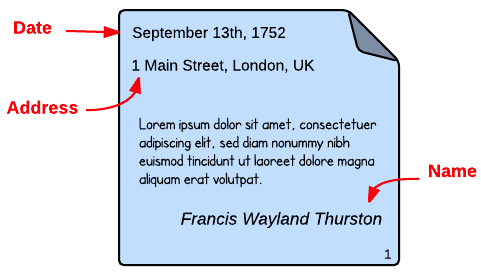
\includegraphics{imgs/text-classification.png}
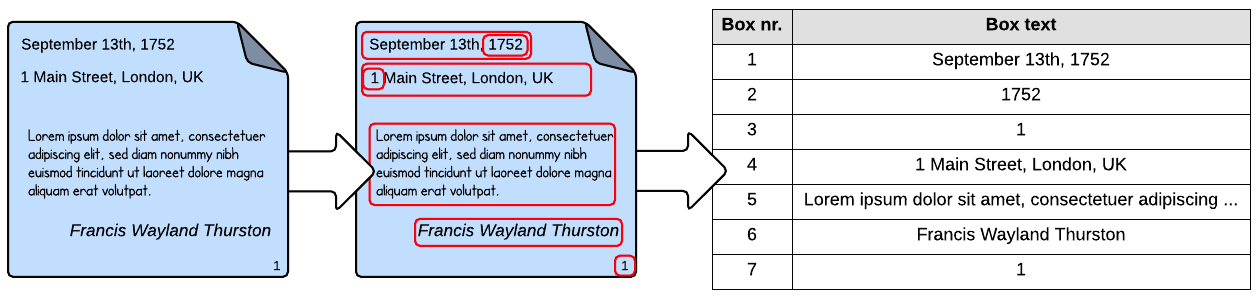
\includegraphics{imgs/text-classification-2.png}

    \hypertarget{datasets-and-inputs}{%
\subsubsection{Datasets and Inputs}\label{datasets-and-inputs}}

The files with the dataset used for this capstone is on the
\href{https://www.kaggle.com/c/tradeshift-text-classification}{link} in
the section Data. We have 4 files on the link, all in the csv format
with a 1-row header and each row stores a different sample and each
collumn is separeted with comma: - \textbf{train.csv}, contains all
features for the training set; - \textbf{trainLabels.csv}, contains one
row per label per sample and the order of the rows is the align with the
train.csv; - \textbf{test.csv}, contains all features for the testing
set; - \textbf{sampleSubmission.csv}, contains a sample submission to
the kaggle competition.

This dataset has \textasciitilde{}2.1M samples with 80\% as training set
and 20\% as the testing set, compounding of 145 features and having 33
labels to classify. The test set is split into public (30\%) and private
(70\%) sets, which are used for the public and the private leaderboard
on the competition. The features of the dataset goes to one of these
categories: - \textbf{Content}: The cryptographic hash of the raw text.
- \textbf{Parsing}: Indicates if the text parses as number, text,
alphanumeric, etc. - \textbf{Spatial}: Indicates the box position, size,
etc. - \textbf{Relational}: Includes information about the surrounding
text blocks in the original document. If there is not such a surrounding
text block, e.g.~a text block in the top of the document does not have
any other text block upper than itself, these features are empty
(no-value).

The feature values can be: - \textbf{Numbers}. Continuous/discrete
numerical values. - \textbf{Boolean}. The values include YES (true) or
NO (false). - \textbf{Categorical}. Values within a finite set of
possible values.

Some observations: * The order of samples and features is random. In
fact, two consecutive samples in the table will most likely not belong
to the same document. * Some documents are OCR'ed; hence, some noise in
the data is expected. * The documents have different formats and the
text belongs to several languages. * The number of pages and text blocks
per document is not constant. * The meaning of the features and class is
not provided.

    \hypertarget{data-exploration}{%
\subsubsection{Data Exploration}\label{data-exploration}}

\begin{enumerate}
\def\labelenumi{\arabic{enumi}.}
\tightlist
\item
  Section \ref{loading_data}
\item
  Section \ref{first_look}
\item
  Section \ref{metadata}
\item
  Section \ref{descriptive}
\item
  Section \ref{quality_check}
\end{enumerate}

    \hypertarget{loading-data}{%
\paragraph{Loading Data }\label{loading-data}}

    \begin{Verbatim}[commandchars=\\\{\}]
{\color{incolor}In [{\color{incolor}1}]:} \PY{o}{\PYZpc{}}\PY{k}{load\PYZus{}ext} autoreload
        \PY{o}{\PYZpc{}}\PY{k}{autoreload} 2
        
        \PY{k+kn}{import} \PY{n+nn}{src}\PY{n+nn}{.}\PY{n+nn}{describe} \PY{k}{as} \PY{n+nn}{d}
        \PY{k+kn}{import} \PY{n+nn}{pandas} \PY{k}{as} \PY{n+nn}{pd}
        
        \PY{n}{pd}\PY{o}{.}\PY{n}{set\PYZus{}option}\PY{p}{(}\PY{l+s+s1}{\PYZsq{}}\PY{l+s+s1}{display.max\PYZus{}columns}\PY{l+s+s1}{\PYZsq{}}\PY{p}{,} \PY{k+kc}{None}\PY{p}{)}  
        \PY{n}{pd}\PY{o}{.}\PY{n}{set\PYZus{}option}\PY{p}{(}\PY{l+s+s1}{\PYZsq{}}\PY{l+s+s1}{display.expand\PYZus{}frame\PYZus{}repr}\PY{l+s+s1}{\PYZsq{}}\PY{p}{,} \PY{k+kc}{False}\PY{p}{)}
        \PY{n}{pd}\PY{o}{.}\PY{n}{set\PYZus{}option}\PY{p}{(}\PY{l+s+s1}{\PYZsq{}}\PY{l+s+s1}{max\PYZus{}colwidth}\PY{l+s+s1}{\PYZsq{}}\PY{p}{,} \PY{o}{\PYZhy{}}\PY{l+m+mi}{1}\PY{p}{)}
        
        \PY{n}{train\PYZus{}features} \PY{o}{=} \PY{n}{d}\PY{o}{.}\PY{n}{read\PYZus{}train\PYZus{}features}\PY{p}{(}\PY{p}{)}
\end{Verbatim}


    \hypertarget{first-look}{%
\paragraph{First look }\label{first-look}}

    \begin{Verbatim}[commandchars=\\\{\}]
{\color{incolor}In [{\color{incolor}2}]:} \PY{n}{train\PYZus{}features}\PY{o}{.}\PY{n}{shape}
\end{Verbatim}


\begin{Verbatim}[commandchars=\\\{\}]
{\color{outcolor}Out[{\color{outcolor}2}]:} (1700000, 146)
\end{Verbatim}
            
    \begin{Verbatim}[commandchars=\\\{\}]
{\color{incolor}In [{\color{incolor}3}]:} \PY{n}{train\PYZus{}features}\PY{o}{.}\PY{n}{head}\PY{p}{(}\PY{p}{)}
\end{Verbatim}


\begin{Verbatim}[commandchars=\\\{\}]
{\color{outcolor}Out[{\color{outcolor}3}]:}    id   x1   x2                                            x3                                            x4        x5        x6        x7        x8        x9  x10  x11  x12  x13  x14  x15       x16  x17  x18       x19  x20   x21   x22   x23  x24  x25  x26  x27       x28       x29 x30 x31  x32  x33                                           x34                                           x35       x36       x37       x38       x39       x40  x41 x42  x43 x44  x45  x46       x47  x48  x49       x50  x51   x52   x53   x54  x55 x56  x57  x58       x59       x60                                           x61  x62 x63                                           x64                                           x65       x66       x67       x68       x69       x70  x71 x72 x73 x74 x75  x76       x77  x78  x79       x80  x81   x82   x83   x84  x85 x86  x87  x88       x89       x90                                           x91  x92 x93                                           x94                                           x95       x96       x97       x98       x99      x100 x101 x102 x103 x104 x105  x106      x107  x108  x109      x110  x111  x112  x113  x114 x115 x116 x117  x118      x119      x120      x121      x122      x123      x124      x125 x126 x127 x128 x129 x130  x131      x132  x133  x134      x135  x136   x137  x138  x139 x140 x141 x142  x143      x144      x145
        0  1   NO   NO   dqOiM6yBYgnVSezBRiQXs9bvOFnRqrtIoXRIElxD7g8=  GNjrXXA3SxbgD0dTRblAPO9jFJ7AIaZnu/f48g5XSUk=  0.576561  0.073139  0.481394  0.115697  0.472474  YES  NO   NO   NO   NO   42   0.396065  3    6    0.991018  0.0  0.82  3306  4676  YES  NO   YES  0    0.405047  0.464610  NO  NO  NO   NO   mimucPmJSF6NI6KM6cPIaaVxWaQyIQzSgtwTTb9bKlc=  s7mTY62CCkWUFc36AW2TlYAy5CIcniD2Vz+lHzyYCLg=  0.576561  0.073139  0.481394  0.115697  0.458560  YES  NO  YES  NO  NO   9    0.368263  2    10   0.992729  0.0  0.94  3306  4676  YES  NO  YES  1    0.375535  0.451301  +2TNtXRI6r9owdGCS80Ia9VVv8ZpuOpVaHEvxRGGu78=  NO   NO  Op+X3asn5H7EQJErI7PR0NkUs3YB+Ld/8OfWuiOC8tU=  GeerC2BbPUcQfQO86NmvOsKrfTvmW7HF+Iru9y+7DPA=  0.576561  0.073139  0.481394  0.115697  0.487598  YES  NO  NO  NO  NO  42   0.363131  6    10   0.987596  0.0  0.71  3306  4676  YES  NO  YES  0    0.375535  0.479734  bxU52teuxC05EZyzFihSiKHczE2ZAIVCXekVLG7j3C0=  NO   NO  +dia7tCOijlRGbABX0YKG5L85x/hXLyJwwplN5Qab04=  f4Uu1R9nnf/h03aqiRQT0Fw3WItzNToLCyRlW1Pn8Z8=  0.576561  0.073139  0.481394  0.115697  0.473079  YES  NO   NO   NO   NO   37    0.333618  4     6     0.987169  0.0   0.89  3306  4676  YES  NO   YES  1     0.346450  0.464610  0.576561  0.073139  0.481394  0.115697  0.473079  YES  NO   NO   NO   NO   42    0.363131  5     6     0.987596  0.0   0.810  3306  4676  YES  NO   YES  2     0.375535  0.464610
        1  2   NaN  NaN  NaN                                           NaN                                           0.000000  0.000000  0.000000  0.000000  0.000000  NaN  NaN  NaN  NaN  NaN  0    0.000000  0    0    0.000000  0.0  0.00  0     0     NaN  NaN  NaN  0    0.000000  0.000000  NO  NO  NO   NO   l0G2rvmLGE6mpPtAibFsoW/0SiNnAuyAc4k35TrHvoQ=  lblNNeOLanWhqgISofUngPYP0Ne1yQv3QeNHqCAoh48=  1.058379  0.125832  0.932547  0.663037  0.569047  YES  NO  NO   NO  NO   9    0.709921  5    6    0.968240  0.0  0.81  4678  3306  YES  NO  YES  3    0.741682  0.560282  MZZbXga8gvaCBqWpzrh2iKdOkcsz/bG/z4BVjUnqWT0=  NO   NO  TqL9cs8ZFzALzVpZv6wYBDi+6zwhrdarQE/3FH+XAlA=  aZTF/lredyP4cukeN8bh6kpBjYmS1QFNpPOg2LVm3Lg=  1.058379  0.125832  0.932547  0.663037  0.628474  YES  NO  NO  NO  NO  2    0.679371  8    7    0.937387  0.0  0.84  4678  3306  YES  NO  YES  1    0.741984  0.619282  YvZUuCDjLu9VvkCdBWgARWQrvm+FSXgxp0zIrMjcLBc=  NO   NO  dsyhxXKNNJy4WVGD/v4+UGyW3jHWkx2xTdg3STsf34A=  X6dDAI/DZOWvu0Dg6gCgRoNr2vTUz/mc4SdHTNUPS38=  1.058379  0.125832  0.932547  0.663037  0.602394  NO   NO   NO   NO   NO   11    0.581367  3     6     0.966122  0.0   0.87  4678  3306  NO   NO   NO   3     0.615245  0.593630  1.058379  0.125832  0.932547  0.663037  0.602394  YES  NO   NO   NO   NO   9     0.709921  4     6     0.968240  0.0   0.510  4678  3306  YES  NO   YES  4     0.741682  0.593630
        2  3   NO   NO   ib4VpsEsqJHzDiyL0dZLQ+xQzDPrkxE+9T3mx5fv2wI=  X6dDAI/DZOWvu0Dg6gCgRoNr2vTUz/mc4SdHTNUPS38=  1.341803  0.051422  0.935572  0.041440  0.501710  NO   NO   YES  NO   NO   2    0.838475  3    5    0.966122  0.0  0.74  4678  3306  NO   NO   NO   2    0.872353  0.493159  NO  NO  YES  YES  9TRXThP/ifDpJRGFX1LQseibUA1NJ3XM53gy+1eZ46k=  XSJ6E8aAoZC7/KAu3eETpfMg3mCq7HVBFIVIsoMKh9E=  1.341803  0.051422  0.935572  0.041440  0.447627  YES  NO  NO   NO  YES  2    0.752269  5    7    0.954930  0.0  0.82  4678  3306  YES  NO  YES  2    0.797338  0.438435  cr+kkNnNFV9YL0vz029hk3ohIDmGuABRVNhFe0ePZyo=  NO   NO  oFsUwSLCWcj8UA1cqILh5afKVcvwlFA+ohJ147Wkz5I=  WV5vAHFyqkeuyFB5KVNGFOBuwjkUGKYc8wh9QfpVzAA=  1.341803  0.051422  0.935572  0.041440  0.522873  YES  NO  NO  NO  NO  1    0.732305  6    6    0.954930  0.0  0.80  4678  3306  YES  NO  YES  0    0.777374  0.513681  X6dDAI/DZOWvu0Dg6gCgRoNr2vTUz/mc4SdHTNUPS38=  NO   NO  mRPnGiKVOWTk/vzZaqlLXZRtdrkcQ/sX0hqBCqOuKq0=  oo9tGpHvTredpg9JkHgYbZAuxcwtSpQxU5mA/zUbxY8=  1.341803  0.051422  0.935572  0.041440  0.501710  NO   NO   NO   NO   NO   2     0.657290  6     5     0.936479  0.0   0.79  4678  3306  NO   NO   NO   0     0.720811  0.493159  1.341803  0.051422  0.935572  0.041440  0.501710  NO   NO   YES  NO   NO   5     0.742589  3     5     0.966122  0.0   0.850  4678  3306  NO   NO   NO   1     0.776467  0.493159
        3  4   YES  NO   BfrqME7vdLw3suQp6YAT16W2piNUmpKhMzuDrVrFQ4w=  YGCdISifn4fLao/ASKdZFhGIq23oqzfSbUVb6px1pig=  0.653912  0.041471  0.940787  0.090851  0.556564  YES  NO   NO   NO   NO   37   0.127405  8    15   0.959171  0.0  0.96  3306  4678  YES  NO   YES  1    0.168234  0.546582  NO  NO  YES  NO   BfrqME7vdLw3suQp6YAT16W2piNUmpKhMzuDrVrFQ4w=  YGCdISifn4fLao/ASKdZFhGIq23oqzfSbUVb6px1pig=  0.653912  0.041471  0.940787  0.090851  0.556564  YES  NO  NO   NO  NO   37   0.127405  8    15   0.959171  0.0  0.96  3306  4678  YES  NO  YES  1    0.168234  0.546582  XQG0f+jmjLI0UHAXXH2RYL4MEHa+yd9okO+730PCZuc=  YES  NO  /1yAAEg6Qib4GMD+wvGOlGmpCIPIAzioWtcCwbns9/I=  YGCdISifn4fLao/ASKdZFhGIq23oqzfSbUVb6px1pig=  0.653912  0.041471  0.940787  0.090851  0.557774  YES  NO  NO  NO  NO  22   0.067764  8    15   0.959598  0.0  0.93  3306  4678  YES  NO  YES  2    0.108166  0.547792  Vl+TDNSupucNoI+Fqeo7bMCkxg1hRjgTSS6NYb9BW00=  YES  NO  /1yAAEg6Qib4GMD+wvGOlGmpCIPIAzioWtcCwbns9/I=  YGCdISifn4fLao/ASKdZFhGIq23oqzfSbUVb6px1pig=  0.653912  0.041471  0.940787  0.090851  0.557774  YES  NO   NO   NO   NO   22    0.067764  8     15    0.959598  0.0   0.93  3306  4678  YES  NO   YES  2     0.108166  0.547792  0.653912  0.041471  0.940787  0.090851  0.557774  YES  NO   NO   NO   NO   0     0.067764  17    15    0.927550  0.0   0.945  3306  4678  NO   NO   YES  3     0.168234  0.546582
        4  5   NO   NO   RTjsrrR8DTlJyaIP9Q3Z8s0zseqlVQTrlSe97GCWfbk=  3yK2OPj1uYDsoMgsxsjY1FxXkOllD8Xfh20VYGqT+nU=  1.415919  0.000000  1.000000  0.000000  0.375297  NO   NO   YES  NO   NO   1    0.523543  4    11   0.963004  0.0  1.00  1263  892   NO   NO   NO   2    0.560538  0.361045  NO  NO  NO   NO   XEDyQD4da6aJkZiBf+r7LD2VdhLGnCMsSpuRFUyCZgg=  Co/nVSLofrWsM5qpcKLXfekegArokgN29XjEXttuXK4=  1.415919  0.000000  1.000000  0.000000  0.300079  YES  NO  NO   NO  YES  6    0.167040  3    3    0.971973  0.0  1.00  1263  892   YES  NO  YES  1    0.195067  0.285827  wIHg6aGH2GMPX6l1pCTzeS1bXE4jxRqmd9ubES4HgW8=  NO   NO  ST8+q2Jgb91pWEwLwmSoJzXEGsQKeQGbzlLbgHPtj4w=  rB07AAHPffU4zFFF8IrqfKSltyWcPyy4+q+IM5SLZiQ=  1.415919  0.000000  1.000000  0.000000  0.400633  NO   NO  NO  NO  NO  9    0.144619  10   14   0.944507 -0.5  1.00  1263  892   NO   NO  NO   1    0.221973  0.386382  WYQEP5EEzM+P+nfkHKLkGko/S3RdBgfEQ3IcyYwrChE=  NO   NO  fylJzYvYlM0+kRBeLB3eFKKgCibqxFvBa8hL+WStwCE=  IoM2E9pNxABFR+H3yfapUL+ThKm7GtTzY7js9H/H99o=  1.415919  0.000000  1.000000  0.000000  0.375297  NO   NO   NO   NO   NO   1     0.065022  8     11    0.927130  0.0   1.00  1263  892   NO   NO   NO   0     0.137892  0.361045  1.415919  0.000000  1.000000  0.000000  0.375297  NO   NO   NO   NO   NO   9     0.146861  11    11    0.900224  0.0   1.000  1263  892   NO   NO   NO   1     0.246637  0.361045
\end{Verbatim}
            
    \begin{Verbatim}[commandchars=\\\{\}]
{\color{incolor}In [{\color{incolor}4}]:} \PY{n}{train\PYZus{}features}\PY{o}{.}\PY{n}{info}\PY{p}{(}\PY{p}{)}
\end{Verbatim}


    \begin{Verbatim}[commandchars=\\\{\}]
<class 'pandas.core.frame.DataFrame'>
RangeIndex: 1700000 entries, 0 to 1699999
Columns: 146 entries, id to x145
dtypes: float64(55), int64(31), object(60)
memory usage: 1.8+ GB

    \end{Verbatim}

    \hypertarget{metadata}{%
\paragraph{Metadata }\label{metadata}}

In this section, we will categorize the collumns to try to facilitate
the manipulation. We'll store: * \textbf{dtype}: int, float, str *
\textbf{category}: content, numerical, boolean

    \begin{Verbatim}[commandchars=\\\{\}]
{\color{incolor}In [{\color{incolor}5}]:} \PY{n}{meta} \PY{o}{=} \PY{n}{d}\PY{o}{.}\PY{n}{create\PYZus{}features\PYZus{}meta}\PY{p}{(}\PY{n}{train\PYZus{}features}\PY{p}{)}
        \PY{n}{meta}\PY{o}{.}\PY{n}{head}\PY{p}{(}\PY{l+m+mi}{10}\PY{p}{)}
\end{Verbatim}


\begin{Verbatim}[commandchars=\\\{\}]
{\color{outcolor}Out[{\color{outcolor}5}]:}           role   category    dtype
        varname                           
        id       id     numerical  int64  
        x1       input  boolean    object 
        x2       input  boolean    object 
        x3       input  content    object 
        x4       input  content    object 
        x5       input  numerical  float64
        x6       input  numerical  float64
        x7       input  numerical  float64
        x8       input  numerical  float64
        x9       input  numerical  float64
\end{Verbatim}
            
    Extract all boolean features:

    \begin{Verbatim}[commandchars=\\\{\}]
{\color{incolor}In [{\color{incolor}6}]:} \PY{n}{meta}\PY{p}{[}\PY{n}{meta}\PY{o}{.}\PY{n}{category} \PY{o}{==} \PY{l+s+s1}{\PYZsq{}}\PY{l+s+s1}{boolean}\PY{l+s+s1}{\PYZsq{}}\PY{p}{]}\PY{o}{.}\PY{n}{index}
\end{Verbatim}


\begin{Verbatim}[commandchars=\\\{\}]
{\color{outcolor}Out[{\color{outcolor}6}]:} Index(['x1', 'x2', 'x10', 'x11', 'x12', 'x13', 'x14', 'x24', 'x25', 'x26',
               'x30', 'x31', 'x32', 'x33', 'x41', 'x42', 'x43', 'x44', 'x45', 'x55',
               'x56', 'x57', 'x62', 'x63', 'x71', 'x72', 'x73', 'x74', 'x75', 'x85',
               'x86', 'x87', 'x92', 'x93', 'x101', 'x102', 'x103', 'x104', 'x105',
               'x115', 'x116', 'x117', 'x126', 'x127', 'x128', 'x129', 'x130', 'x140',
               'x141', 'x142'],
              dtype='object', name='varname')
\end{Verbatim}
            
    See the quantity of feature per category:

    \begin{Verbatim}[commandchars=\\\{\}]
{\color{incolor}In [{\color{incolor}7}]:} \PY{n}{pd}\PY{o}{.}\PY{n}{DataFrame}\PY{p}{(}\PY{p}{\PYZob{}}\PY{l+s+s1}{\PYZsq{}}\PY{l+s+s1}{count}\PY{l+s+s1}{\PYZsq{}} \PY{p}{:} \PY{n}{meta}\PY{o}{.}\PY{n}{groupby}\PY{p}{(}\PY{p}{[}\PY{l+s+s1}{\PYZsq{}}\PY{l+s+s1}{category}\PY{l+s+s1}{\PYZsq{}}\PY{p}{,} \PY{l+s+s1}{\PYZsq{}}\PY{l+s+s1}{dtype}\PY{l+s+s1}{\PYZsq{}}\PY{p}{]}\PY{p}{)}\PY{p}{[}\PY{l+s+s1}{\PYZsq{}}\PY{l+s+s1}{dtype}\PY{l+s+s1}{\PYZsq{}}\PY{p}{]}\PY{o}{.}\PY{n}{size}\PY{p}{(}\PY{p}{)}\PY{p}{\PYZcb{}}\PY{p}{)}\PY{o}{.}\PY{n}{reset\PYZus{}index}\PY{p}{(}\PY{p}{)}
\end{Verbatim}


\begin{Verbatim}[commandchars=\\\{\}]
{\color{outcolor}Out[{\color{outcolor}7}]:}     category    dtype  count
        0  boolean    object   50   
        1  content    object   10   
        2  numerical  int64    31   
        3  numerical  float64  55   
\end{Verbatim}
            
    \hypertarget{descriptive-statistics}{%
\paragraph{Descriptive Statistics }\label{descriptive-statistics}}

In this section we will apply the \emph{describe} method on the features
splited by category and dtype to calculate the mean, standart deviation,
max, min\ldots{}

\textbf{\emph{Numerical float variables}}

    \begin{Verbatim}[commandchars=\\\{\}]
{\color{incolor}In [{\color{incolor}8}]:} \PY{n}{float\PYZus{}features} \PY{o}{=} \PY{n}{meta}\PY{p}{[}\PY{p}{(}\PY{n}{meta}\PY{o}{.}\PY{n}{category} \PY{o}{==} \PY{l+s+s1}{\PYZsq{}}\PY{l+s+s1}{numerical}\PY{l+s+s1}{\PYZsq{}}\PY{p}{)} \PY{o}{\PYZam{}} \PY{p}{(}\PY{n}{meta}\PY{o}{.}\PY{n}{dtype} \PY{o}{==} \PY{l+s+s1}{\PYZsq{}}\PY{l+s+s1}{float64}\PY{l+s+s1}{\PYZsq{}}\PY{p}{)}\PY{p}{]}\PY{o}{.}\PY{n}{index}
        \PY{n}{float\PYZus{}train\PYZus{}features} \PY{o}{=} \PY{n}{train\PYZus{}features}\PY{p}{[}\PY{n}{float\PYZus{}features}\PY{p}{]}
        \PY{n}{float\PYZus{}train\PYZus{}features\PYZus{}describe} \PY{o}{=} \PY{n}{float\PYZus{}train\PYZus{}features}\PY{o}{.}\PY{n}{describe}\PY{p}{(}\PY{p}{)}
        \PY{n}{float\PYZus{}train\PYZus{}features\PYZus{}describe}
\end{Verbatim}


\begin{Verbatim}[commandchars=\\\{\}]
{\color{outcolor}Out[{\color{outcolor}8}]:}                  x5            x6            x7            x8            x9           x16           x19           x20           x21           x28           x29           x36           x37           x38           x39           x40           x47           x50           x51           x52           x59           x60           x66           x67           x68           x69           x70           x77           x80           x81           x82           x89           x90           x96           x97           x98           x99          x100          x107          x110          x111          x112          x119          x120          x121          x122          x123          x124          x125          x132          x135          x136          x137          x144          x145
        count  1.700000e+06  1.700000e+06  1.700000e+06  1.700000e+06  1.700000e+06  1.700000e+06  1.700000e+06  1.700000e+06  1.700000e+06  1.700000e+06  1.700000e+06  1.700000e+06  1.700000e+06  1.700000e+06  1.700000e+06  1.700000e+06  1.700000e+06  1.700000e+06  1.700000e+06  1.700000e+06  1.700000e+06  1.700000e+06  1.700000e+06  1.700000e+06  1.700000e+06  1.700000e+06  1.700000e+06  1.700000e+06  1.700000e+06  1.700000e+06  1.700000e+06  1.700000e+06  1.700000e+06  1.700000e+06  1.700000e+06  1.700000e+06  1.700000e+06  1.700000e+06  1.700000e+06  1.700000e+06  1.700000e+06  1.700000e+06  1.700000e+06  1.700000e+06  1.700000e+06  1.700000e+06  1.700000e+06  1.700000e+06  1.700000e+06  1.700000e+06  1.700000e+06  1.700000e+06  1.700000e+06  1.700000e+06  1.700000e+06
        mean   9.551493e-01  5.531406e-02  7.906443e-01  1.731225e-01  4.462953e-01  4.196774e-01  8.185989e-01 -6.392546e-02  7.858669e-01  4.523190e-01  4.378473e-01  1.082852e+00  6.117782e-02  8.954949e-01  1.830648e-01  4.846973e-01  4.348303e-01  9.112922e-01 -8.473989e-02  8.910999e-01  4.898810e-01  4.749733e-01  1.082232e+00  6.106558e-02  8.841590e-01  1.989396e-01  5.124087e-01  4.270050e-01  8.953298e-01 -8.269609e-02  8.798031e-01  4.870141e-01  5.029204e-01  1.027301e+00  5.602975e-02  8.466713e-01  1.833974e-01  4.780893e-01  3.693654e-01  8.783841e-01 -6.801648e-02  8.460217e-01  4.053633e-01  4.689895e-01  1.121410e+00  6.366866e-02  9.229534e-01  1.967985e-01  5.163925e-01  4.397928e-01  9.336593e-01  7.678663e-02  9.231219e-01  5.238243e-01  5.053399e-01
        std    5.278641e-01  1.318832e-01  3.549407e-01  3.326885e-01  3.026847e-01  2.945485e-01  3.422650e-01  4.972203e-01  3.457971e-01  3.019166e-01  3.010004e-01  4.222894e-01  1.369235e-01  2.233018e-01  3.280037e-01  2.633006e-01  2.817998e-01  1.892331e-01  6.268609e-01  2.024930e-01  2.823276e-01  2.633976e-01  4.265242e-01  1.365560e-01  2.422241e-01  3.513484e-01  2.731636e-01  2.850214e-01  2.214036e-01  6.064530e-01  2.234765e-01  2.869244e-01  2.727644e-01  4.761280e-01  1.275268e-01  2.958083e-01  3.368791e-01  2.857023e-01  2.660854e-01  2.688927e-01  5.270641e-01  2.804542e-01  2.673060e-01  2.848163e-01  3.789949e-01  1.397335e-01  1.604844e-01  3.432269e-01  2.577492e-01  2.781111e-01  7.191982e-02  1.538817e+00  1.215640e-01  2.703335e-01  2.582544e-01
        min    0.000000e+00  0.000000e+00  0.000000e+00  0.000000e+00 -1.042755e+00 -5.919283e-01 -3.520179e-01 -4.600000e+01  0.000000e+00 -5.762332e-01 -1.051465e+00  0.000000e+00  0.000000e+00  0.000000e+00  0.000000e+00 -1.839272e+00 -6.244395e-01 -4.652466e-01 -4.800000e+01  0.000000e+00 -5.997758e-01 -1.847189e+00  0.000000e+00  0.000000e+00  0.000000e+00  0.000000e+00 -1.839272e+00 -6.244395e-01 -4.652466e-01 -4.800000e+01  0.000000e+00 -5.997758e-01 -1.847189e+00  0.000000e+00  0.000000e+00  0.000000e+00  0.000000e+00 -1.042755e+00 -6.244395e-01 -3.520179e-01 -4.800000e+01  0.000000e+00 -5.997758e-01 -1.051465e+00  0.000000e+00  0.000000e+00  0.000000e+00  0.000000e+00 -2.584323e+00 -6.793722e-01 -3.520179e-01 -4.800000e+01  0.000000e+00 -5.762332e-01 -2.592241e+00
        25\%    6.367211e-01  0.000000e+00  8.438324e-01  0.000000e+00  1.961279e-01  1.670404e-01  9.292196e-01  0.000000e+00  7.900000e-01  2.062780e-01  1.854545e-01  7.068146e-01  0.000000e+00  9.231700e-01  0.000000e+00  2.782293e-01  1.717569e-01  9.327354e-01  0.000000e+00  8.600000e-01  2.331839e-01  2.686212e-01  7.068146e-01  0.000000e+00  9.204477e-01  0.000000e+00  3.056215e-01  1.636771e-01  9.310954e-01  0.000000e+00  8.600000e-01  2.302266e-01  2.955626e-01  6.539119e-01  0.000000e+00  9.056261e-01  0.000000e+00  2.541568e-01  1.267636e-01  9.383872e-01  0.000000e+00  8.500000e-01  1.729664e-01  2.435905e-01  7.879613e-01  0.000000e+00  9.277072e-01  0.000000e+00  3.151227e-01  1.785164e-01  9.162930e-01  0.000000e+00  8.800000e-01  2.756953e-01  3.041061e-01
        50\%    1.270115e+00  0.000000e+00  9.588627e-01  0.000000e+00  4.393339e-01  4.002242e-01  9.630045e-01  0.000000e+00  9.500000e-01  4.433551e-01  4.295221e-01  1.294118e+00  0.000000e+00  1.000000e+00  0.000000e+00  4.632322e-01  4.104658e-01  9.582577e-01  0.000000e+00  1.000000e+00  4.697309e-01  4.536817e-01  1.294118e+00  0.000000e+00  1.000000e+00  0.000000e+00  5.002273e-01  3.976471e-01  9.576656e-01  0.000000e+00  1.000000e+00  4.639082e-01  4.899103e-01  1.294118e+00  0.000000e+00  9.788328e-01  0.000000e+00  4.656831e-01  3.279412e-01  9.652466e-01  0.000000e+00  9.800000e-01  3.721973e-01  4.560570e-01  1.296128e+00  0.000000e+00  1.000000e+00  0.000000e+00  4.957192e-01  4.170404e-01  9.495516e-01  0.000000e+00  1.000000e+00  5.235426e-01  4.843750e-01
        75\%    1.414798e+00  5.837871e-02  1.000000e+00  1.451906e-01  6.866182e-01  6.822070e-01  9.809417e-01  0.000000e+00  1.000000e+00  7.197309e-01  6.767036e-01  1.414798e+00  6.624319e-02  1.000000e+00  2.001202e-01  6.844131e-01  6.894619e-01  9.758016e-01  0.000000e+00  1.000000e+00  7.387773e-01  6.750069e-01  1.414798e+00  6.594071e-02  1.000000e+00  2.177858e-01  7.390960e-01  6.863479e-01  9.760349e-01  0.000000e+00  1.000000e+00  7.432735e-01  7.292162e-01  1.414798e+00  6.295400e-02  1.000000e+00  1.800000e-01  7.049960e-01  6.095830e-01  9.814708e-01  0.000000e+00  1.000000e+00  6.479412e-01  6.952862e-01  1.414798e+00  6.836056e-02  1.000000e+00  2.212130e-01  7.247429e-01  6.905830e-01  9.725093e-01  0.000000e+00  1.000000e+00  7.640909e-01  7.132486e-01
        max    2.732124e+00  9.987901e-01  1.000000e+00  1.753333e+00  1.942155e+00  7.929372e+00  9.997862e-01  1.400000e+01  1.000000e+00  7.968610e+00  1.932647e+00  2.732124e+00  9.982420e-01  1.000000e+00  1.753333e+00  1.942155e+00  3.884529e+00  9.997862e-01  1.400000e+01  1.000000e+00  3.923767e+00  1.932647e+00  2.732124e+00  9.982420e-01  1.000000e+00  1.793262e+00  1.942155e+00  3.884529e+00  9.997862e-01  9.333333e+00  1.000000e+00  3.923767e+00  1.932647e+00  2.732124e+00  9.953120e-01  1.000000e+00  1.753333e+00  1.942155e+00  7.929372e+00  9.997862e-01  1.400000e+01  1.000000e+00  7.968610e+00  1.932647e+00  2.732124e+00  9.982420e-01  1.000000e+00  1.753333e+00  1.942155e+00  7.974215e+00  9.999985e-01  1.470000e+02  1.000000e+00  8.002242e+00  1.932647e+00
\end{Verbatim}
            
    \begin{Verbatim}[commandchars=\\\{\}]
{\color{incolor}In [{\color{incolor}9}]:} \PY{n}{float\PYZus{}train\PYZus{}features\PYZus{}describe}\PY{o}{.}\PY{n}{loc}\PY{p}{(}\PY{p}{)}\PY{p}{[}\PY{p}{[}\PY{l+s+s1}{\PYZsq{}}\PY{l+s+s1}{min}\PY{l+s+s1}{\PYZsq{}}\PY{p}{,}\PY{l+s+s1}{\PYZsq{}}\PY{l+s+s1}{max}\PY{l+s+s1}{\PYZsq{}}\PY{p}{]}\PY{p}{]}
\end{Verbatim}


\begin{Verbatim}[commandchars=\\\{\}]
{\color{outcolor}Out[{\color{outcolor}9}]:}            x5       x6   x7        x8        x9       x16       x19   x20  x21       x28       x29       x36       x37  x38       x39       x40       x47       x50   x51  x52       x59       x60       x66       x67  x68       x69       x70       x77       x80        x81  x82       x89       x90       x96       x97  x98       x99      x100      x107      x110  x111  x112      x119      x120      x121      x122  x123      x124      x125      x132      x135   x136  x137      x144      x145
        min  0.000000  0.00000  0.0  0.000000 -1.042755 -0.591928 -0.352018 -46.0  0.0 -0.576233 -1.051465  0.000000  0.000000  0.0  0.000000 -1.839272 -0.624439 -0.465247 -48.0  0.0 -0.599776 -1.847189  0.000000  0.000000  0.0  0.000000 -1.839272 -0.624439 -0.465247 -48.000000  0.0 -0.599776 -1.847189  0.000000  0.000000  0.0  0.000000 -1.042755 -0.624439 -0.352018 -48.0  0.0  -0.599776 -1.051465  0.000000  0.000000  0.0   0.000000 -2.584323 -0.679372 -0.352018 -48.0   0.0  -0.576233 -2.592241
        max  2.732124  0.99879  1.0  1.753333  1.942155  7.929372  0.999786  14.0  1.0  7.968610  1.932647  2.732124  0.998242  1.0  1.753333  1.942155  3.884529  0.999786  14.0  1.0  3.923767  1.932647  2.732124  0.998242  1.0  1.793262  1.942155  3.884529  0.999786  9.333333   1.0  3.923767  1.932647  2.732124  0.995312  1.0  1.753333  1.942155  7.929372  0.999786  14.0  1.0   7.968610  1.932647  2.732124  0.998242  1.0   1.753333  1.942155  7.974215  0.999998  147.0  1.0   8.002242  1.932647
\end{Verbatim}
            
    \begin{Verbatim}[commandchars=\\\{\}]
{\color{incolor}In [{\color{incolor}10}]:} \PY{n}{float\PYZus{}train\PYZus{}features}\PY{o}{.}\PY{n}{isnull}\PY{p}{(}\PY{p}{)}\PY{o}{.}\PY{n}{any}\PY{p}{(}\PY{p}{)}\PY{o}{.}\PY{n}{any}\PY{p}{(}\PY{p}{)}
\end{Verbatim}


\begin{Verbatim}[commandchars=\\\{\}]
{\color{outcolor}Out[{\color{outcolor}10}]:} False
\end{Verbatim}
            
    The features that are scaled between {[}0,1{]} are: x6, x7, x21, x37,
x38, x52, x67, x68, x82, x97, x98, x112, x122, x123, x137.

So we could apply scaling on the other features depends on the
classifier.

And we don't have any NaN values on this features.

    \textbf{\emph{Numerical int variables}}

    \begin{Verbatim}[commandchars=\\\{\}]
{\color{incolor}In [{\color{incolor}11}]:} \PY{n}{int\PYZus{}features} \PY{o}{=} \PY{n}{meta}\PY{p}{[}\PY{p}{(}\PY{n}{meta}\PY{o}{.}\PY{n}{category} \PY{o}{==} \PY{l+s+s1}{\PYZsq{}}\PY{l+s+s1}{numerical}\PY{l+s+s1}{\PYZsq{}}\PY{p}{)} \PY{o}{\PYZam{}} \PY{p}{(}\PY{n}{meta}\PY{o}{.}\PY{n}{dtype} \PY{o}{==} \PY{l+s+s1}{\PYZsq{}}\PY{l+s+s1}{int64}\PY{l+s+s1}{\PYZsq{}}\PY{p}{)}\PY{p}{]}\PY{o}{.}\PY{n}{index}
         \PY{n}{int\PYZus{}train\PYZus{}features} \PY{o}{=} \PY{n}{train\PYZus{}features}\PY{p}{[}\PY{n}{int\PYZus{}features}\PY{p}{]}
         \PY{n}{int\PYZus{}train\PYZus{}features\PYZus{}describe} \PY{o}{=} \PY{n}{int\PYZus{}train\PYZus{}features}\PY{o}{.}\PY{n}{describe}\PY{p}{(}\PY{p}{)}
         \PY{n}{int\PYZus{}train\PYZus{}features\PYZus{}describe}
\end{Verbatim}


\begin{Verbatim}[commandchars=\\\{\}]
{\color{outcolor}Out[{\color{outcolor}11}]:}                  id           x15           x17           x18           x22           x23           x27           x46           x48           x49           x53           x54           x58           x76           x78           x79           x83           x84           x88          x106          x108          x109          x113          x114          x118          x131          x133          x134          x138          x139          x143
         count  1.700000e+06  1.700000e+06  1.700000e+06  1.700000e+06  1.700000e+06  1.700000e+06  1.700000e+06  1.700000e+06  1.700000e+06  1.700000e+06  1.700000e+06  1.700000e+06  1.700000e+06  1.700000e+06  1.700000e+06  1.700000e+06  1.700000e+06  1.700000e+06  1.700000e+06  1.700000e+06  1.700000e+06  1.700000e+06  1.700000e+06  1.700000e+06  1.700000e+06  1.700000e+06  1.700000e+06  1.700000e+06  1.700000e+06  1.700000e+06  1.700000e+06
         mean   8.500005e+05  6.154404e+00  4.487084e+00  8.096322e+00  2.301595e+03  1.874765e+03  2.814097e+00  8.151020e+00  6.973005e+00  8.363310e+00  2.605915e+03  2.098133e+03  2.640614e+00  8.259205e+00  7.502141e+00  8.401614e+00  2.581685e+03  2.079391e+03  2.685396e+00  7.851039e+00  4.854556e+00  8.419647e+00  2.469781e+03  1.998761e+03  2.314082e+00  4.809295e+00  9.301809e+00  8.842868e+00  2.688457e+03  2.163423e+03  3.632134e+00
         std    4.907479e+05  8.957511e+00  4.623426e+00  7.123864e+00  1.745120e+03  1.517991e+03  4.409801e+00  1.036050e+01  9.311837e+00  6.656968e+00  1.632477e+03  1.421664e+03  3.823310e+00  1.055778e+01  1.129549e+01  6.834330e+00  1.648193e+03  1.433160e+03  3.921535e+00  1.001937e+01  4.483374e+00  6.886586e+00  1.691323e+03  1.470973e+03  3.914509e+00  8.966942e+00  7.725215e+00  6.665332e+00  1.591809e+03  1.392787e+03  9.424120e+00
         min    1.000000e+00  0.000000e+00  0.000000e+00  0.000000e+00  0.000000e+00  0.000000e+00 -1.000000e+00  0.000000e+00  0.000000e+00  0.000000e+00  0.000000e+00  0.000000e+00 -1.000000e+00  0.000000e+00  0.000000e+00  0.000000e+00  0.000000e+00  0.000000e+00 -1.000000e+00  0.000000e+00  0.000000e+00  0.000000e+00  0.000000e+00  0.000000e+00 -1.000000e+00  0.000000e+00  0.000000e+00  0.000000e+00  0.000000e+00  0.000000e+00 -1.000000e+00
         25\%    4.250008e+05  1.000000e+00  2.000000e+00  3.000000e+00  1.261000e+03  8.920000e+02  0.000000e+00  2.000000e+00  3.000000e+00  4.000000e+00  1.262000e+03  8.920000e+02  0.000000e+00  2.000000e+00  3.000000e+00  4.000000e+00  1.262000e+03  8.920000e+02  0.000000e+00  2.000000e+00  2.000000e+00  4.000000e+00  1.261000e+03  8.920000e+02  0.000000e+00  0.000000e+00  4.000000e+00  4.000000e+00  1.262000e+03  8.920000e+02  1.000000e+00
         50\%    8.500005e+05  3.000000e+00  4.000000e+00  7.000000e+00  1.263000e+03  8.920000e+02  1.000000e+00  4.000000e+00  5.000000e+00  7.000000e+00  1.263000e+03  9.180000e+02  1.000000e+00  4.000000e+00  5.000000e+00  7.000000e+00  1.263000e+03  9.180000e+02  1.000000e+00  4.000000e+00  4.000000e+00  7.000000e+00  1.263000e+03  9.180000e+02  1.000000e+00  1.000000e+00  7.000000e+00  7.000000e+00  1.263000e+03  9.180000e+02  2.000000e+00
         75\%    1.275000e+06  7.000000e+00  6.000000e+00  1.100000e+01  4.400000e+03  3.307000e+03  4.000000e+00  9.000000e+00  8.000000e+00  1.100000e+01  4.659000e+03  3.307000e+03  4.000000e+00  9.000000e+00  8.000000e+00  1.200000e+01  4.643000e+03  3.307000e+03  4.000000e+00  9.000000e+00  7.000000e+00  1.200000e+01  4.400000e+03  3.307000e+03  3.000000e+00  5.000000e+00  1.300000e+01  1.200000e+01  4.672000e+03  3.308000e+03  5.000000e+00
         max    1.700000e+06  1.530000e+02  2.370000e+02  2.190000e+02  1.950000e+04  1.416700e+04  6.720000e+02  1.530000e+02  3.710000e+02  2.190000e+02  1.950000e+04  1.416700e+04  3.370000e+02  1.530000e+02  2.710000e+02  2.190000e+02  1.950000e+04  1.416700e+04  2.840000e+02  1.530000e+02  2.430000e+02  2.190000e+02  1.950000e+04  1.416700e+04  4.100000e+02  1.530000e+02  3.010000e+02  2.190000e+02  1.950000e+04  1.416700e+04  1.219000e+03
\end{Verbatim}
            
    \begin{Verbatim}[commandchars=\\\{\}]
{\color{incolor}In [{\color{incolor}12}]:} \PY{n}{int\PYZus{}train\PYZus{}features\PYZus{}describe}\PY{o}{.}\PY{n}{loc}\PY{p}{(}\PY{p}{)}\PY{p}{[}\PY{p}{[}\PY{l+s+s1}{\PYZsq{}}\PY{l+s+s1}{min}\PY{l+s+s1}{\PYZsq{}}\PY{p}{,}\PY{l+s+s1}{\PYZsq{}}\PY{l+s+s1}{max}\PY{l+s+s1}{\PYZsq{}}\PY{p}{]}\PY{p}{]}
\end{Verbatim}


\begin{Verbatim}[commandchars=\\\{\}]
{\color{outcolor}Out[{\color{outcolor}12}]:}             id    x15    x17    x18      x22      x23    x27    x46    x48    x49      x53      x54    x58    x76    x78    x79      x83      x84    x88   x106   x108   x109     x113     x114   x118   x131   x133   x134     x138     x139    x143
         min  1.0        0.0    0.0    0.0    0.0      0.0     -1.0    0.0    0.0    0.0    0.0      0.0     -1.0    0.0    0.0    0.0    0.0      0.0     -1.0    0.0    0.0    0.0    0.0      0.0     -1.0    0.0    0.0    0.0    0.0      0.0     -1.0   
         max  1700000.0  153.0  237.0  219.0  19500.0  14167.0  672.0  153.0  371.0  219.0  19500.0  14167.0  337.0  153.0  271.0  219.0  19500.0  14167.0  284.0  153.0  243.0  219.0  19500.0  14167.0  410.0  153.0  301.0  219.0  19500.0  14167.0  1219.0
\end{Verbatim}
            
    \begin{Verbatim}[commandchars=\\\{\}]
{\color{incolor}In [{\color{incolor}13}]:} \PY{n}{int\PYZus{}train\PYZus{}features\PYZus{}describe}\PY{o}{.}\PY{n}{isnull}\PY{p}{(}\PY{p}{)}\PY{o}{.}\PY{n}{any}\PY{p}{(}\PY{p}{)}\PY{o}{.}\PY{n}{any}\PY{p}{(}\PY{p}{)}
\end{Verbatim}


\begin{Verbatim}[commandchars=\\\{\}]
{\color{outcolor}Out[{\color{outcolor}13}]:} False
\end{Verbatim}
            
    All the int numerical features are not scaled, so depending on the
algorithm we have to scale the feature, we don't have any missing value.
The problem here is we don't know when the feature is a categorical
feature or a quantitative.

    \textbf{\emph{Content variables}}

    \begin{Verbatim}[commandchars=\\\{\}]
{\color{incolor}In [{\color{incolor}14}]:} \PY{n}{content\PYZus{}features} \PY{o}{=} \PY{n}{meta}\PY{p}{[}\PY{p}{(}\PY{n}{meta}\PY{o}{.}\PY{n}{category} \PY{o}{==} \PY{l+s+s1}{\PYZsq{}}\PY{l+s+s1}{content}\PY{l+s+s1}{\PYZsq{}}\PY{p}{)}\PY{p}{]}\PY{o}{.}\PY{n}{index}
         \PY{n}{content\PYZus{}train\PYZus{}features} \PY{o}{=} \PY{n}{train\PYZus{}features}\PY{p}{[}\PY{n}{content\PYZus{}features}\PY{p}{]}
         \PY{n}{content\PYZus{}train\PYZus{}features\PYZus{}describe} \PY{o}{=} \PY{n}{content\PYZus{}train\PYZus{}features}\PY{o}{.}\PY{n}{describe}\PY{p}{(}\PY{p}{)}
         \PY{n}{content\PYZus{}train\PYZus{}features\PYZus{}describe}
\end{Verbatim}


\begin{Verbatim}[commandchars=\\\{\}]
{\color{outcolor}Out[{\color{outcolor}14}]:}                                                   x3                                            x4                                           x34                                           x35                                           x61                                           x64                                           x65                                           x91                                           x94                                           x95
         count   1451737                                       1451737                                       1649154                                       1649154                                       1699968                                       1628939                                       1628939                                       1699968                                       1559381                                       1559381                                     
         unique  201881                                        26428                                         241245                                        35700                                         461141                                        245418                                        36814                                         134998                                        184925                                        26791                                       
         top     MZZbXga8gvaCBqWpzrh2iKdOkcsz/bG/z4BVjUnqWT0=  hCXwO/JldK5zcd9ejOD1FwmEgCf96eTdEVy7OtY2Y2g=  MZZbXga8gvaCBqWpzrh2iKdOkcsz/bG/z4BVjUnqWT0=  YvZUuCDjLu9VvkCdBWgARWQrvm+FSXgxp0zIrMjcLBc=  X/hdUOVR5KuExVGLzjhLcM2CyIqym9t0Nh+ZX05M+1w=  MZZbXga8gvaCBqWpzrh2iKdOkcsz/bG/z4BVjUnqWT0=  YvZUuCDjLu9VvkCdBWgARWQrvm+FSXgxp0zIrMjcLBc=  +yhSY//Hpg7u0bSA7NYmcmRFgv3bF4Tw3BMHrBqaTtA=  MZZbXga8gvaCBqWpzrh2iKdOkcsz/bG/z4BVjUnqWT0=  hCXwO/JldK5zcd9ejOD1FwmEgCf96eTdEVy7OtY2Y2g=
         freq    51212                                         86750                                         57978                                         84162                                         60369                                         65666                                         93540                                         89494                                         47700                                         105073                                      
\end{Verbatim}
            
    \begin{Verbatim}[commandchars=\\\{\}]
{\color{incolor}In [{\color{incolor}15}]:} \PY{n}{uniques} \PY{o}{=} \PY{n+nb}{set}\PY{p}{(}\PY{p}{)}
         \PY{k}{for} \PY{n}{c} \PY{o+ow}{in} \PY{n}{content\PYZus{}train\PYZus{}features}\PY{o}{.}\PY{n}{columns}\PY{p}{:}
             \PY{n}{uniques}\PY{o}{.}\PY{n}{update}\PY{p}{(}\PY{n}{content\PYZus{}train\PYZus{}features}\PY{p}{[}\PY{n}{c}\PY{p}{]}\PY{o}{.}\PY{n}{unique}\PY{p}{(}\PY{p}{)}\PY{o}{.}\PY{n}{tolist}\PY{p}{(}\PY{p}{)}\PY{p}{)}
         \PY{n+nb}{print}\PY{p}{(}\PY{l+s+s1}{\PYZsq{}}\PY{l+s+s1}{total uniques words=}\PY{l+s+si}{\PYZob{}\PYZcb{}}\PY{l+s+s1}{\PYZsq{}}\PY{o}{.}\PY{n}{format}\PY{p}{(}\PY{n+nb}{len}\PY{p}{(}\PY{n}{uniques}\PY{p}{)}\PY{p}{)}\PY{p}{)}
         
         \PY{c+c1}{\PYZsh{} flattening all the words to count them}
         \PY{n}{all\PYZus{}words} \PY{o}{=} \PY{n}{pd}\PY{o}{.}\PY{n}{Series}\PY{p}{(}\PY{n}{content\PYZus{}train\PYZus{}features}\PY{o}{.}\PY{n}{values}\PY{o}{.}\PY{n}{flatten}\PY{p}{(}\PY{l+s+s1}{\PYZsq{}}\PY{l+s+s1}{F}\PY{l+s+s1}{\PYZsq{}}\PY{p}{)}\PY{p}{)}
         \PY{n}{all\PYZus{}words} \PY{o}{=} \PY{n}{all\PYZus{}words}\PY{o}{.}\PY{n}{to\PYZus{}frame}\PY{p}{(}\PY{p}{)}\PY{o}{.}\PY{n}{reset\PYZus{}index}\PY{p}{(}\PY{p}{)}
         \PY{n+nb}{print}\PY{p}{(}\PY{l+s+s1}{\PYZsq{}}\PY{l+s+s1}{total words=}\PY{l+s+si}{\PYZob{}\PYZcb{}}\PY{l+s+s1}{\PYZsq{}}\PY{o}{.}\PY{n}{format}\PY{p}{(}\PY{n}{all\PYZus{}words}\PY{o}{.}\PY{n}{shape}\PY{p}{[}\PY{l+m+mi}{0}\PY{p}{]}\PY{p}{)}\PY{p}{)}
         \PY{n}{all\PYZus{}words} \PY{o}{=} \PY{n}{all\PYZus{}words}\PY{o}{.}\PY{n}{rename}\PY{p}{(}\PY{n}{columns}\PY{o}{=} \PY{p}{\PYZob{}}\PY{l+m+mi}{0}\PY{p}{:} \PY{l+s+s1}{\PYZsq{}}\PY{l+s+s1}{words}\PY{l+s+s1}{\PYZsq{}}\PY{p}{\PYZcb{}}\PY{p}{)}
         \PY{n}{all\PYZus{}words} \PY{o}{=} \PY{n}{pd}\PY{o}{.}\PY{n}{DataFrame}\PY{p}{(}\PY{p}{\PYZob{}}\PY{l+s+s1}{\PYZsq{}}\PY{l+s+s1}{count}\PY{l+s+s1}{\PYZsq{}} \PY{p}{:} \PY{n}{all\PYZus{}words}\PY{o}{.}\PY{n}{groupby}\PY{p}{(}\PY{p}{[}\PY{l+s+s1}{\PYZsq{}}\PY{l+s+s1}{words}\PY{l+s+s1}{\PYZsq{}}\PY{p}{]}\PY{p}{)}\PY{p}{[}\PY{l+s+s1}{\PYZsq{}}\PY{l+s+s1}{words}\PY{l+s+s1}{\PYZsq{}}\PY{p}{]}\PY{o}{.}\PY{n}{size}\PY{p}{(}\PY{p}{)}\PY{p}{\PYZcb{}}\PY{p}{)}\PY{o}{.}\PY{n}{reset\PYZus{}index}\PY{p}{(}\PY{p}{)}
         \PY{n}{all\PYZus{}words}\PY{o}{.}\PY{n}{sort\PYZus{}values}\PY{p}{(}\PY{l+s+s1}{\PYZsq{}}\PY{l+s+s1}{count}\PY{l+s+s1}{\PYZsq{}}\PY{p}{,} \PY{n}{ascending}\PY{o}{=}\PY{k+kc}{False}\PY{p}{)}\PY{o}{.}\PY{n}{head}\PY{p}{(}\PY{l+m+mi}{10}\PY{p}{)}
\end{Verbatim}


    \begin{Verbatim}[commandchars=\\\{\}]
total uniques words=979749
total words=17000000

    \end{Verbatim}

\begin{Verbatim}[commandchars=\\\{\}]
{\color{outcolor}Out[{\color{outcolor}15}]:}                                                words   count
         565834  YvZUuCDjLu9VvkCdBWgARWQrvm+FSXgxp0zIrMjcLBc=  392698
         538278  X6dDAI/DZOWvu0Dg6gCgRoNr2vTUz/mc4SdHTNUPS38=  356811
         692301  hCXwO/JldK5zcd9ejOD1FwmEgCf96eTdEVy7OtY2Y2g=  317031
         376725  MZZbXga8gvaCBqWpzrh2iKdOkcsz/bG/z4BVjUnqWT0=  273502
         199214  B+EJpnEbkYtLnwDQYN1dP1rcfnoCnxAjKLYwQZE07Ew=  260233
         15027   +yhSY//Hpg7u0bSA7NYmcmRFgv3bF4Tw3BMHrBqaTtA=  260166
         528829  WV5vAHFyqkeuyFB5KVNGFOBuwjkUGKYc8wh9QfpVzAA=  237367
         264280  FExKgjj6CsbToTubdZ+kGsOmUx3gCvZVJCdZPcdPNF4=  208934
         808722  oo9tGpHvTredpg9JkHgYbZAuxcwtSpQxU5mA/zUbxY8=  182455
         49401   1CiKJR7D66tRwH6l6wwv0p+D/tAuoW+NdSNqPTbvDoQ=  176907
\end{Verbatim}
            
    \begin{Verbatim}[commandchars=\\\{\}]
{\color{incolor}In [{\color{incolor}16}]:} \PY{n}{content\PYZus{}train\PYZus{}features}\PY{o}{.}\PY{n}{isnull}\PY{p}{(}\PY{p}{)}\PY{o}{.}\PY{n}{sum}\PY{p}{(}\PY{p}{)}
\end{Verbatim}


\begin{Verbatim}[commandchars=\\\{\}]
{\color{outcolor}Out[{\color{outcolor}16}]:} x3     248263
         x4     248263
         x34    50846 
         x35    50846 
         x61    32    
         x64    71061 
         x65    71061 
         x91    32    
         x94    140619
         x95    140619
         dtype: int64
\end{Verbatim}
            
    On the hashed words we have 979\_749 unique words on 17\_000\_000 (1.7kk
rows x 10 collumns) words giving 5.76\% of uniques words on the total
words. This show us that word can have a huge impact on the classifier
because we have some words multiples times. But we have to take care of
the NaN values and treat them.

    \textbf{\emph{Boolean variables}}

    \begin{Verbatim}[commandchars=\\\{\}]
{\color{incolor}In [{\color{incolor}17}]:} \PY{n}{bool\PYZus{}vars} \PY{o}{=} \PY{n}{meta}\PY{p}{[}\PY{p}{(}\PY{n}{meta}\PY{o}{.}\PY{n}{category} \PY{o}{==} \PY{l+s+s1}{\PYZsq{}}\PY{l+s+s1}{boolean}\PY{l+s+s1}{\PYZsq{}}\PY{p}{)}\PY{p}{]}\PY{o}{.}\PY{n}{index}
         \PY{n}{train\PYZus{}features}\PY{p}{[}\PY{n}{bool\PYZus{}vars}\PY{p}{]}\PY{o}{.}\PY{n}{describe}\PY{p}{(}\PY{p}{)}
         \PY{n}{train\PYZus{}features}\PY{p}{[}\PY{n}{bool\PYZus{}vars}\PY{p}{]}\PY{o}{.}\PY{n}{isnull}\PY{p}{(}\PY{p}{)}\PY{o}{.}\PY{n}{sum}\PY{p}{(}\PY{p}{)}
\end{Verbatim}


\begin{Verbatim}[commandchars=\\\{\}]
{\color{outcolor}Out[{\color{outcolor}17}]:} x1      248190
         x2      248190
         x10     248263
         x11     248263
         x12     248263
         x13     248263
         x14     248263
         x24     248263
         x25     248263
         x26     248263
         x30     0     
         x31     0     
         x32     50772 
         x33     50772 
         x41     50846 
         x42     50846 
         x43     50846 
         x44     50846 
         x45     50846 
         x55     50846 
         x56     50846 
         x57     50846 
         x62     70978 
         x63     70978 
         x71     71061 
         x72     71061 
         x73     71061 
         x74     71061 
         x75     71061 
         x85     71061 
         x86     71061 
         x87     71061 
         x92     140526
         x93     140526
         x101    140619
         x102    140619
         x103    140619
         x104    140619
         x105    140619
         x115    140619
         x116    140619
         x117    140619
         x126    32    
         x127    32    
         x128    32    
         x129    32    
         x130    32    
         x140    32    
         x141    32    
         x142    32    
         dtype: int64
\end{Verbatim}
            
    On the boolean values, only on 2 features we have no missing values. So
we have to treat all this missing values here.

    \hypertarget{data-quality-checks}{%
\paragraph{Data Quality Checks }\label{data-quality-checks}}

\textbf{\emph{Checking Missings Values}}

    \begin{Verbatim}[commandchars=\\\{\}]
{\color{incolor}In [{\color{incolor}18}]:} \PY{n}{vars\PYZus{}with\PYZus{}missing} \PY{o}{=} \PY{p}{[}\PY{p}{]}
         \PY{k}{for} \PY{n}{f} \PY{o+ow}{in} \PY{n}{train\PYZus{}features}\PY{o}{.}\PY{n}{columns}\PY{p}{:}
             \PY{n}{missings} \PY{o}{=} \PY{n}{train\PYZus{}features}\PY{p}{[}\PY{n}{f}\PY{p}{]}\PY{o}{.}\PY{n}{isnull}\PY{p}{(}\PY{p}{)}\PY{o}{.}\PY{n}{sum}\PY{p}{(}\PY{p}{)}
             \PY{k}{if} \PY{n}{missings} \PY{o}{\PYZgt{}} \PY{l+m+mi}{0}\PY{p}{:}
                 \PY{n}{vars\PYZus{}with\PYZus{}missing}\PY{o}{.}\PY{n}{append}\PY{p}{(}\PY{n}{f}\PY{p}{)}
                 \PY{n}{missings\PYZus{}perc} \PY{o}{=} \PY{n}{missings}\PY{o}{/}\PY{n}{train\PYZus{}features}\PY{o}{.}\PY{n}{shape}\PY{p}{[}\PY{l+m+mi}{0}\PY{p}{]}
                 \PY{n}{category} \PY{o}{=} \PY{n}{meta}\PY{o}{.}\PY{n}{loc}\PY{p}{[}\PY{n}{f}\PY{p}{]}\PY{p}{[}\PY{l+s+s1}{\PYZsq{}}\PY{l+s+s1}{category}\PY{l+s+s1}{\PYZsq{}}\PY{p}{]}
                 \PY{n}{dtype} \PY{o}{=} \PY{n}{meta}\PY{o}{.}\PY{n}{loc}\PY{p}{[}\PY{n}{f}\PY{p}{]}\PY{p}{[}\PY{l+s+s1}{\PYZsq{}}\PY{l+s+s1}{dtype}\PY{l+s+s1}{\PYZsq{}}\PY{p}{]}
                 
                 \PY{n+nb}{print}\PY{p}{(}\PY{l+s+s1}{\PYZsq{}}\PY{l+s+s1}{Variable }\PY{l+s+si}{\PYZob{}\PYZcb{}}\PY{l+s+s1}{ (}\PY{l+s+si}{\PYZob{}\PYZcb{}}\PY{l+s+s1}{, }\PY{l+s+si}{\PYZob{}\PYZcb{}}\PY{l+s+s1}{) has }\PY{l+s+si}{\PYZob{}\PYZcb{}}\PY{l+s+s1}{ records (}\PY{l+s+si}{\PYZob{}:.2\PYZpc{}\PYZcb{}}\PY{l+s+s1}{) with missing values}\PY{l+s+s1}{\PYZsq{}}\PY{o}{.}\PY{n}{format}\PY{p}{(}\PY{n}{f}\PY{p}{,} \PY{n}{category}\PY{p}{,} \PY{n}{dtype}\PY{p}{,} \PY{n}{missings}\PY{p}{,} \PY{n}{missings\PYZus{}perc}\PY{p}{)}\PY{p}{)}
                 
         \PY{n+nb}{print}\PY{p}{(}\PY{l+s+s1}{\PYZsq{}}\PY{l+s+s1}{In total, there are }\PY{l+s+si}{\PYZob{}\PYZcb{}}\PY{l+s+s1}{ variables with missing values}\PY{l+s+s1}{\PYZsq{}}\PY{o}{.}\PY{n}{format}\PY{p}{(}\PY{n+nb}{len}\PY{p}{(}\PY{n}{vars\PYZus{}with\PYZus{}missing}\PY{p}{)}\PY{p}{)}\PY{p}{)}
\end{Verbatim}


    \begin{Verbatim}[commandchars=\\\{\}]
Variable x1 (boolean, object) has 248190 records (14.60\%) with missing values
Variable x2 (boolean, object) has 248190 records (14.60\%) with missing values
Variable x3 (content, object) has 248263 records (14.60\%) with missing values
Variable x4 (content, object) has 248263 records (14.60\%) with missing values
Variable x10 (boolean, object) has 248263 records (14.60\%) with missing values
Variable x11 (boolean, object) has 248263 records (14.60\%) with missing values
Variable x12 (boolean, object) has 248263 records (14.60\%) with missing values
Variable x13 (boolean, object) has 248263 records (14.60\%) with missing values
Variable x14 (boolean, object) has 248263 records (14.60\%) with missing values
Variable x24 (boolean, object) has 248263 records (14.60\%) with missing values
Variable x25 (boolean, object) has 248263 records (14.60\%) with missing values
Variable x26 (boolean, object) has 248263 records (14.60\%) with missing values
Variable x32 (boolean, object) has 50772 records (2.99\%) with missing values
Variable x33 (boolean, object) has 50772 records (2.99\%) with missing values
Variable x34 (content, object) has 50846 records (2.99\%) with missing values
Variable x35 (content, object) has 50846 records (2.99\%) with missing values
Variable x41 (boolean, object) has 50846 records (2.99\%) with missing values
Variable x42 (boolean, object) has 50846 records (2.99\%) with missing values
Variable x43 (boolean, object) has 50846 records (2.99\%) with missing values
Variable x44 (boolean, object) has 50846 records (2.99\%) with missing values
Variable x45 (boolean, object) has 50846 records (2.99\%) with missing values
Variable x55 (boolean, object) has 50846 records (2.99\%) with missing values
Variable x56 (boolean, object) has 50846 records (2.99\%) with missing values
Variable x57 (boolean, object) has 50846 records (2.99\%) with missing values
Variable x61 (content, object) has 32 records (0.00\%) with missing values
Variable x62 (boolean, object) has 70978 records (4.18\%) with missing values
Variable x63 (boolean, object) has 70978 records (4.18\%) with missing values
Variable x64 (content, object) has 71061 records (4.18\%) with missing values
Variable x65 (content, object) has 71061 records (4.18\%) with missing values
Variable x71 (boolean, object) has 71061 records (4.18\%) with missing values
Variable x72 (boolean, object) has 71061 records (4.18\%) with missing values
Variable x73 (boolean, object) has 71061 records (4.18\%) with missing values
Variable x74 (boolean, object) has 71061 records (4.18\%) with missing values
Variable x75 (boolean, object) has 71061 records (4.18\%) with missing values
Variable x85 (boolean, object) has 71061 records (4.18\%) with missing values
Variable x86 (boolean, object) has 71061 records (4.18\%) with missing values
Variable x87 (boolean, object) has 71061 records (4.18\%) with missing values
Variable x91 (content, object) has 32 records (0.00\%) with missing values
Variable x92 (boolean, object) has 140526 records (8.27\%) with missing values
Variable x93 (boolean, object) has 140526 records (8.27\%) with missing values
Variable x94 (content, object) has 140619 records (8.27\%) with missing values
Variable x95 (content, object) has 140619 records (8.27\%) with missing values
Variable x101 (boolean, object) has 140619 records (8.27\%) with missing values
Variable x102 (boolean, object) has 140619 records (8.27\%) with missing values
Variable x103 (boolean, object) has 140619 records (8.27\%) with missing values
Variable x104 (boolean, object) has 140619 records (8.27\%) with missing values
Variable x105 (boolean, object) has 140619 records (8.27\%) with missing values
Variable x115 (boolean, object) has 140619 records (8.27\%) with missing values
Variable x116 (boolean, object) has 140619 records (8.27\%) with missing values
Variable x117 (boolean, object) has 140619 records (8.27\%) with missing values
Variable x126 (boolean, object) has 32 records (0.00\%) with missing values
Variable x127 (boolean, object) has 32 records (0.00\%) with missing values
Variable x128 (boolean, object) has 32 records (0.00\%) with missing values
Variable x129 (boolean, object) has 32 records (0.00\%) with missing values
Variable x130 (boolean, object) has 32 records (0.00\%) with missing values
Variable x140 (boolean, object) has 32 records (0.00\%) with missing values
Variable x141 (boolean, object) has 32 records (0.00\%) with missing values
Variable x142 (boolean, object) has 32 records (0.00\%) with missing values
In total, there are 58 variables with missing values

    \end{Verbatim}

    \textbf{\emph{Checking the cardinality of the int variables}}

Cardinality means the differents values of a variable, so we will see
which feature will became dummy variables.

    \begin{Verbatim}[commandchars=\\\{\}]
{\color{incolor}In [{\color{incolor}19}]:} \PY{k}{for} \PY{n}{f} \PY{o+ow}{in} \PY{n}{int\PYZus{}train\PYZus{}features}\PY{p}{:}
             \PY{n}{dist\PYZus{}values} \PY{o}{=} \PY{n}{int\PYZus{}train\PYZus{}features}\PY{p}{[}\PY{n}{f}\PY{p}{]}\PY{o}{.}\PY{n}{value\PYZus{}counts}\PY{p}{(}\PY{p}{)}\PY{o}{.}\PY{n}{shape}\PY{p}{[}\PY{l+m+mi}{0}\PY{p}{]}
             \PY{n+nb}{print}\PY{p}{(}\PY{l+s+s1}{\PYZsq{}}\PY{l+s+s1}{Variable }\PY{l+s+si}{\PYZob{}\PYZcb{}}\PY{l+s+s1}{ has }\PY{l+s+si}{\PYZob{}\PYZcb{}}\PY{l+s+s1}{ distinct values}\PY{l+s+s1}{\PYZsq{}}\PY{o}{.}\PY{n}{format}\PY{p}{(}\PY{n}{f}\PY{p}{,} \PY{n}{dist\PYZus{}values}\PY{p}{)}\PY{p}{)}
\end{Verbatim}


    \begin{Verbatim}[commandchars=\\\{\}]
Variable id has 1700000 distinct values
Variable x15 has 97 distinct values
Variable x17 has 119 distinct values
Variable x18 has 108 distinct values
Variable x22 has 498 distinct values
Variable x23 has 419 distinct values
Variable x27 has 193 distinct values
Variable x46 has 122 distinct values
Variable x48 has 167 distinct values
Variable x49 has 110 distinct values
Variable x53 has 499 distinct values
Variable x54 has 419 distinct values
Variable x58 has 149 distinct values
Variable x76 has 127 distinct values
Variable x78 has 184 distinct values
Variable x79 has 109 distinct values
Variable x83 has 498 distinct values
Variable x84 has 417 distinct values
Variable x88 has 141 distinct values
Variable x106 has 109 distinct values
Variable x108 has 123 distinct values
Variable x109 has 109 distinct values
Variable x113 has 500 distinct values
Variable x114 has 419 distinct values
Variable x118 has 159 distinct values
Variable x131 has 125 distinct values
Variable x133 has 158 distinct values
Variable x134 has 110 distinct values
Variable x138 has 500 distinct values
Variable x139 has 420 distinct values
Variable x143 has 493 distinct values

    \end{Verbatim}

    At this point i can't see if I will treat this variables as categorical
and transform in dummy variables or treat them as quatitative variables.

    \hypertarget{solution-statement}{%
\subsubsection{Solution Statement}\label{solution-statement}}

The solution proposed is to train a classifier to predict the labels of
the extract OCR and the features created by the Tradeshift using the
negative logarithm of the likelihood function to estimate the score for
the classifier.

    \hypertarget{benchmark-model}{%
\subsubsection{Benchmark Model}\label{benchmark-model}}

In this competition, the organizers give us fours different benchmarks
scores: * The all zeros benchmark, where every label answer is zero; *
The random benchmark, where every label was given a random value; * The
halves benchmark, where every label was given a value of 0.5; * And
finally the Tradeshift Baseline Benchmark.

The score of the four benchmarks is find below, in this evaluation
metric lower is better:

\begin{longtable}[]{@{}ll@{}}
\toprule
Benchmark & Score\tabularnewline
\midrule
\endhead
TS Baseline & 0.0150548\tabularnewline
All Halves & 0.6931471\tabularnewline
Random & 1.0122952\tabularnewline
All Zeros & 1.1706929\tabularnewline
\bottomrule
\end{longtable}

    \hypertarget{evaluation-metrics}{%
\subsubsection{Evaluation Metrics}\label{evaluation-metrics}}

The evaluation metric chosen by the organizers was the negative
logarithm of the likelihood function averaged over Nt test samples and K
labels. As shown by the following equation a + b =c. On the equation:

    \begin{Verbatim}[commandchars=\\\{\}]
{\color{incolor}In [{\color{incolor}48}]:} \PY{c}{\PYZpc{}\PYZpc{}latex}
         \PY{l+s+sb}{\PYZdl{}\PYZdl{}}\PY{n+nv}{\PYZbs{}textrm}\PY{n+nb}{\PYZob{}}\PY{n+nb}{LogLoss}\PY{n+nb}{\PYZcb{}}\PY{n+nb}{ }\PY{o}{=}\PY{n+nb}{ }\PY{n+nv}{\PYZbs{}frac}\PY{n+nb}{\PYZob{}}\PY{l+m}{1}\PY{n+nb}{\PYZcb{}}\PY{n+nb}{\PYZob{}}\PY{n+nb}{N}\PY{n+nb}{\PYZus{}}\PY{n+nb}{\PYZob{}}\PY{n+nb}{t}\PY{n+nb}{\PYZcb{}}\PY{n+nb}{ }\PY{n+nv}{\PYZbs{}cdot}\PY{n+nb}{ K}\PY{n+nb}{\PYZcb{}}\PY{n+nb}{ }\PY{n+nv}{\PYZbs{}sum}\PY{n+nb}{\PYZus{}}\PY{n+nb}{\PYZob{}}\PY{n+nb}{idx}\PY{o}{=}\PY{l+m}{1}\PY{n+nb}{\PYZcb{}}\PY{n+nb}{\PYZca{}}\PY{n+nb}{\PYZob{}}\PY{n+nb}{N}\PY{n+nb}{\PYZus{}}\PY{n+nb}{\PYZob{}}\PY{n+nb}{t}\PY{n+nb}{\PYZcb{}}\PY{n+nb}{ }\PY{n+nv}{\PYZbs{}cdot}\PY{n+nb}{ K}\PY{n+nb}{\PYZcb{}}\PY{n+nb}{ }\PY{n+nv}{\PYZbs{}textrm}\PY{n+nb}{\PYZob{}}\PY{n+nb}{LogLoss}\PY{n+nb}{\PYZcb{}}\PY{n+nb}{\PYZus{}}\PY{n+nb}{\PYZob{}}\PY{n+nb}{idx}\PY{n+nb}{\PYZcb{}}\PY{l+s}{\PYZdl{}\PYZdl{}}
         \PY{l+s+sb}{\PYZdl{}\PYZdl{}}\PY{o}{=}\PY{n+nb}{ }\PY{n+nv}{\PYZbs{}frac}\PY{n+nb}{\PYZob{}}\PY{l+m}{1}\PY{n+nb}{\PYZcb{}}\PY{n+nb}{\PYZob{}}\PY{n+nb}{N}\PY{n+nb}{\PYZus{}}\PY{n+nb}{\PYZob{}}\PY{n+nb}{t}\PY{n+nb}{\PYZcb{}}\PY{n+nb}{ }\PY{n+nv}{\PYZbs{}cdot}\PY{n+nb}{ K}\PY{n+nb}{\PYZcb{}}\PY{n+nb}{ }\PY{n+nv}{\PYZbs{}sum}\PY{n+nb}{\PYZus{}}\PY{n+nb}{\PYZob{}}\PY{n+nb}{idx}\PY{o}{=}\PY{l+m}{1}\PY{n+nb}{\PYZcb{}}\PY{n+nb}{\PYZca{}}\PY{n+nb}{\PYZob{}}\PY{n+nb}{N}\PY{n+nb}{\PYZus{}}\PY{n+nb}{\PYZob{}}\PY{n+nb}{t}\PY{n+nb}{\PYZcb{}}\PY{n+nb}{ }\PY{n+nv}{\PYZbs{}cdot}\PY{n+nb}{ K}\PY{n+nb}{\PYZcb{}}\PY{n+nb}{ }\PY{n+nv}{\PYZbs{}left}\PY{o}{[}\PY{n+nb}{ }\PY{o}{\PYZhy{}}\PY{n+nb}{ y}\PY{n+nb}{\PYZus{}}\PY{n+nb}{\PYZob{}}\PY{n+nb}{idx}\PY{n+nb}{\PYZcb{}}\PY{n+nb}{ }\PY{n+nv}{\PYZbs{}log}\PY{o}{(}\PY{n+nv}{\PYZbs{}hat}\PY{n+nb}{\PYZob{}}\PY{n+nb}{y}\PY{n+nb}{\PYZcb{}}\PY{n+nb}{\PYZus{}}\PY{n+nb}{\PYZob{}}\PY{n+nb}{idx}\PY{n+nb}{\PYZcb{}}\PY{o}{)}\PY{n+nb}{ }\PY{o}{\PYZhy{}}\PY{n+nb}{ }\PY{o}{(}\PY{l+m}{1}\PY{n+nb}{ }\PY{o}{\PYZhy{}}\PY{n+nb}{ y}\PY{n+nb}{\PYZus{}}\PY{n+nb}{\PYZob{}}\PY{n+nb}{idx}\PY{n+nb}{\PYZcb{}}\PY{o}{)}\PY{n+nb}{ }\PY{n+nv}{\PYZbs{}log}\PY{o}{(}\PY{l+m}{1}\PY{n+nb}{ }\PY{o}{\PYZhy{}}\PY{n+nb}{ }\PY{n+nv}{\PYZbs{}hat}\PY{n+nb}{\PYZob{}}\PY{n+nb}{y}\PY{n+nb}{\PYZcb{}}\PY{n+nb}{\PYZus{}}\PY{n+nb}{\PYZob{}}\PY{n+nb}{idx}\PY{n+nb}{\PYZcb{}}\PY{o}{)}\PY{n+nv}{\PYZbs{}right}\PY{o}{]}\PY{l+s}{\PYZdl{}\PYZdl{}}
         \PY{l+s+sb}{\PYZdl{}\PYZdl{}}\PY{o}{=}\PY{n+nb}{ }\PY{n+nv}{\PYZbs{}frac}\PY{n+nb}{\PYZob{}}\PY{l+m}{1}\PY{n+nb}{\PYZcb{}}\PY{n+nb}{\PYZob{}}\PY{n+nb}{N}\PY{n+nb}{\PYZus{}}\PY{n+nb}{\PYZob{}}\PY{n+nb}{t}\PY{n+nb}{\PYZcb{}}\PY{n+nb}{ }\PY{n+nv}{\PYZbs{}cdot}\PY{n+nb}{ K}\PY{n+nb}{\PYZcb{}}\PY{n+nb}{ }\PY{n+nv}{\PYZbs{}sum}\PY{n+nb}{\PYZus{}}\PY{n+nb}{\PYZob{}}\PY{n+nb}{i}\PY{o}{=}\PY{l+m}{1}\PY{n+nb}{\PYZcb{}}\PY{n+nb}{\PYZca{}}\PY{n+nb}{\PYZob{}}\PY{n+nb}{N}\PY{n+nb}{\PYZus{}}\PY{n+nb}{\PYZob{}}\PY{n+nb}{t}\PY{n+nb}{\PYZcb{}}\PY{n+nb}{\PYZcb{}}\PY{n+nb}{ }\PY{n+nv}{\PYZbs{}sum}\PY{n+nb}{\PYZus{}}\PY{n+nb}{\PYZob{}}\PY{n+nb}{j}\PY{o}{=}\PY{l+m}{1}\PY{n+nb}{\PYZcb{}}\PY{n+nb}{\PYZca{}}\PY{n+nb}{K }\PY{n+nv}{\PYZbs{}left}\PY{o}{[}\PY{n+nb}{ }\PY{o}{\PYZhy{}}\PY{n+nb}{ y}\PY{n+nb}{\PYZus{}}\PY{n+nb}{\PYZob{}}\PY{n+nb}{ij}\PY{n+nb}{\PYZcb{}}\PY{n+nb}{ }\PY{n+nv}{\PYZbs{}log}\PY{o}{(}\PY{n+nv}{\PYZbs{}hat}\PY{n+nb}{\PYZob{}}\PY{n+nb}{y}\PY{n+nb}{\PYZcb{}}\PY{n+nb}{\PYZus{}}\PY{n+nb}{\PYZob{}}\PY{n+nb}{ij}\PY{n+nb}{\PYZcb{}}\PY{o}{)}\PY{n+nb}{ }\PY{o}{\PYZhy{}}\PY{n+nb}{ }\PY{o}{(}\PY{l+m}{1}\PY{n+nb}{ }\PY{o}{\PYZhy{}}\PY{n+nb}{ y}\PY{n+nb}{\PYZus{}}\PY{n+nb}{\PYZob{}}\PY{n+nb}{ij}\PY{n+nb}{\PYZcb{}}\PY{o}{)}\PY{n+nb}{ }\PY{n+nv}{\PYZbs{}log}\PY{o}{(}\PY{l+m}{1}\PY{n+nb}{ }\PY{o}{\PYZhy{}}\PY{n+nb}{ }\PY{n+nv}{\PYZbs{}hat}\PY{n+nb}{\PYZob{}}\PY{n+nb}{y}\PY{n+nb}{\PYZcb{}}\PY{n+nb}{\PYZus{}}\PY{n+nb}{\PYZob{}}\PY{n+nb}{ij}\PY{n+nb}{\PYZcb{}}\PY{o}{)}\PY{n+nv}{\PYZbs{}right}\PY{o}{]}\PY{l+s}{\PYZdl{}\PYZdl{}}
\end{Verbatim}


    $$\textrm{LogLoss} = \frac{1}{N_{t} \cdot K} \sum_{idx=1}^{N_{t} \cdot K} \textrm{LogLoss}_{idx}$$
$$= \frac{1}{N_{t} \cdot K} \sum_{idx=1}^{N_{t} \cdot K} \left[ - y_{idx} \log(\hat{y}_{idx}) - (1 - y_{idx}) \log(1 - \hat{y}_{idx})\right]$$
$$= \frac{1}{N_{t} \cdot K} \sum_{i=1}^{N_{t}} \sum_{j=1}^K \left[ - y_{ij} \log(\hat{y}_{ij}) - (1 - y_{ij}) \log(1 - \hat{y}_{ij})\right]$$


    
    \begin{itemize}
\tightlist
\item
  \(f\) is the prediction model
\item
  \(\theta\) is the parameter of the model
\item
  \(\hat{y}_{ij}\) is the predicted probability of the jth-label is true
  for the ith-sample
\item
  \(log\) represents the natural logarithm
\item
  \(idx = (i - 1) * K + j\)
\end{itemize}

This function penalizes probabilities that are confident and wrong, in
the worst case, prediction of true(1) for a false label (0) add infinity
to the LogLoss function as \(-log(0) = \infty\), which makes a total
score infinity regardless of the others scores.

This metric is also symmetric in the sense than predicting 0.1 for a
false (0) sample has the same penalty as predicting 0.9 for a positive
sample (1). The value is bounded between zero and infinity, i.e.
\(\textrm{LogLoss} \in [0, \infty)\). The competition corresponds to a
minimization problem where smaller metric values,
\(\textrm{LogLoss} \sim 0\), implies better prediction models. To avoid
complication with infinity values the predictions are bounded to within
the range \([10^{-15},1-10^{-15}]\)

    \hypertarget{example}{%
\paragraph{Example}\label{example}}

    This is an example from the competition If the `answer' file is:

\begin{verbatim}
id_label,pred
1_y1,1.0000
1_y2,0.0000
1_y3,0.0000
1_y4,0.0000
2_y1,0.0000
2_y2,1.0000
2_y3,0.0000
2_y4,1.0000
3_y1,0.0000
3_y2,0.0000
3_y3,1.0000
3_y4,0.0000
\end{verbatim}

And the submission file is:

\begin{verbatim}
id_label,pred
1_y1,0.9000
1_y2,0.1000
1_y3,0.0000
1_y4,0.3000
2_y1,0.0300
2_y2,0.7000
2_y3,0.2000
2_y4,0.8500
3_y1,0.1900
3_y2,0.0000
3_y3,1.0000
3_y4,0.2700
\end{verbatim}

the score is 0.1555 as shown by:

    \begin{Verbatim}[commandchars=\\\{\}]
{\color{incolor}In [{\color{incolor}2}]:} \PY{c}{\PYZpc{}\PYZpc{}latex}
        \PY{l+s+sb}{\PYZdl{}\PYZdl{}}\PY{n+nb}{L }\PY{o}{=}\PY{n+nb}{ }\PY{o}{\PYZhy{}}\PY{n+nb}{ }\PY{n+nv}{\PYZbs{}frac}\PY{n+nb}{\PYZob{}}\PY{l+m}{1}\PY{n+nb}{\PYZcb{}}\PY{n+nb}{\PYZob{}}\PY{l+m}{12}\PY{n+nb}{\PYZcb{}}\PY{n+nb}{ }\PY{n+nv}{\PYZbs{}left}\PY{n+nb}{ }\PY{o}{[}\PY{n+nb}{ log}\PY{o}{(}\PY{l+m}{0}\PY{n+nb}{.}\PY{l+m}{9}\PY{o}{)}\PY{n+nb}{ }\PY{o}{+}\PY{n+nb}{ log}\PY{o}{(}\PY{l+m}{1}\PY{o}{\PYZhy{}}\PY{l+m}{0}\PY{n+nb}{.}\PY{l+m}{1}\PY{o}{)}\PY{n+nb}{ }\PY{o}{+}\PY{n+nb}{ log}\PY{o}{(}\PY{l+m}{1}\PY{o}{\PYZhy{}}\PY{l+m}{0}\PY{n+nb}{.}\PY{l+m}{0}\PY{o}{)}\PY{n+nb}{ }\PY{o}{+}\PY{n+nb}{log}\PY{o}{(}\PY{l+m}{1}\PY{o}{\PYZhy{}}\PY{l+m}{0}\PY{n+nb}{.}\PY{l+m}{3}\PY{o}{)}\PY{n+nb}{ }\PY{o}{+}\PY{n+nb}{ log}\PY{o}{(}\PY{l+m}{1}\PY{o}{\PYZhy{}}\PY{l+m}{0}\PY{n+nb}{.}\PY{l+m}{03}\PY{o}{)}\PY{n+nb}{ }\PY{o}{+}\PY{n+nb}{ log}\PY{o}{(}\PY{l+m}{0}\PY{n+nb}{.}\PY{l+m}{7}\PY{o}{)}\PY{n+nb}{ }\PY{o}{+}\PY{n+nb}{ log}\PY{o}{(}\PY{l+m}{1}\PY{o}{\PYZhy{}}\PY{l+m}{0}\PY{n+nb}{.}\PY{l+m}{2}\PY{o}{)}\PY{n+nb}{ }\PY{o}{+}\PY{n+nb}{ log}\PY{o}{(}\PY{l+m}{0}\PY{n+nb}{.}\PY{l+m}{85}\PY{o}{)}\PY{n+nb}{ }\PY{o}{+}\PY{n+nb}{ log}\PY{o}{(}\PY{l+m}{1}\PY{o}{\PYZhy{}}\PY{l+m}{0}\PY{n+nb}{.}\PY{l+m}{19}\PY{o}{)}\PY{n+nb}{  }\PY{o}{+}\PY{n+nb}{ log}\PY{o}{(}\PY{l+m}{1}\PY{o}{\PYZhy{}}\PY{l+m}{0}\PY{n+nb}{.}\PY{l+m}{0}\PY{o}{)}\PY{n+nb}{ }\PY{o}{+}\PY{n+nb}{ log}\PY{o}{(}\PY{l+m}{1}\PY{n+nb}{.}\PY{l+m}{0}\PY{o}{)}\PY{n+nb}{ }\PY{o}{+}\PY{n+nb}{log}\PY{o}{(}\PY{l+m}{1}\PY{o}{\PYZhy{}}\PY{l+m}{0}\PY{n+nb}{.}\PY{l+m}{27}\PY{o}{)}\PY{n+nb}{ }\PY{n+nv}{\PYZbs{}right}\PY{n+nb}{ }\PY{o}{]}\PY{n+nb}{ }\PY{o}{=}\PY{n+nb}{ }\PY{l+m}{0}\PY{n+nb}{.}\PY{l+m}{1555}\PY{l+s}{\PYZdl{}\PYZdl{}}
\end{Verbatim}


    $$L = - \frac{1}{12} \left [ log(0.9) + log(1-0.1) + log(1-0.0) +log(1-0.3) + log(1-0.03) + log(0.7) + log(1-0.2) + log(0.85) + log(1-0.19)  + log(1-0.0) + log(1.0) +log(1-0.27) \right ] = 0.1555$$


    
    \hypertarget{project-design}{%
\subsubsection{Project Design}\label{project-design}}

First of all, I will be preprocessing the data for the ingestion on the
classifier, normalizing the numerical features, one-hot encoding the
categorical features, convert of the content variables to a one-hot
encoding and dealing with the invalids and missing entries. After the
preprocessing, I will choose some ensemble methods to test the score and
see what is the most important features from each ensemble method.
Seeing what are the most important features, will train the same
ensemble methods with some variation of the most impactful features like
top 1\%, 5\%, 10\%, 50\% and see what is the quantity of feature has the
most impact on the score. After that can apply a PCA method varying the
number of features and train again the ensemble methods to see if the
feature selection or PCA is the way to go. Passing this phase I can try
to optimize the hyperparameter to the best-supervised learning method I
find in the process above.

    \hypertarget{references}{%
\subsubsection{References}\label{references}}

\begin{itemize}
\tightlist
\item
  {[}0{]} - https://www.kaggle.com/c/tradeshift-text-classification
\item
  {[}1{]} -
  https://en.wikipedia.org/wiki/Optical\_character\_recognition
\item
  {[}2{]} - http://ccis2k.org/iajit/PDF/vol.5,no.1/3-37.pdf - Zakaria
  Elberrichi, Abdelattif Rahmoun, and Mohamed Amine Bentaalah - Using
  WordNet for Text Categorization - The International Arab Journal of
  Information Technology, Vol. 5, No.~1, January 2008
\item
  {[}3{]} - http://odur.let.rug.nl/vannoord/TextCat/textcat.pdf -
  William B. Cavnar and John M. Trenkle - N-Gram-Based Text
  Categorization - Environmental Research Institute of Michigan
\item
  {[}4{]} -
  http://www.ijaiem.org/Volume2Issue3/IJAIEM-2013-03-13-025.pdf -
  Bhumika, Prof Sukhjit Singh Sehra, Prof Anand Nayyar - A REVIEW PAPER
  ON ALGORITHMS USED FOR TEXT CLASSIFICATION - International Journal of
  Application or Innovation in Engineering \& Management (IJAIEM) -
  Volume 2, Issue 3, March 2013
\item
  {[}5{]} -
  https://www.researchgate.net/publication/319688772\_Using\_text\_mining\_to\_classify\_research\_papers
  - Sulova, Snezhana \& Todoranova, Latinka \& Penchev, Bonimir \&
  Nacheva, Radka. (2017). Using text mining to classify research papers.
  10.5593/SGEM2017/21/S07.083.
\item
  {[}6{]} -
  https://www.researchgate.net/publication/280609521\_Text\_Classification\_of\_Technical\_Papers\_Based\_on\_Text\_Segmentation
  - Nguyen, Thien \& Shirai, Kiyoaki. (2013). Text Classification of
  Technical Papers Based on Text Segmentation.
  10.1007/978-3-642-38824-8\_25.
\item
  {[}7{]} -
  https://blog.tradeshift.com/hundreds-compete-to-improve-machine-learning-algorithm-for-5k-prize/
\item
  {[}8{]} -
  https://www.kaggle.com/bertcarremans/data-preparation-exploration
\item
  {[}9{]} -
  https://blog.metaflow.fr/ml-notes-why-the-log-likelihood-24f7b6c40f83
\item
  {[}10{]} -
  https://quantivity.wordpress.com/2011/05/23/why-minimize-negative-log-likelihood/
\end{itemize}


    % Add a bibliography block to the postdoc
    
    
    
    \end{document}
